\documentclass[12pt]{ruthesis}
\usepackage{amsmath}
\usepackage{amssymb}
\usepackage{graphics}
\usepackage{subfigure}
\usepackage{natbib}
%subpackages for marking up changes
\usepackage{soul,color}
\usepackage[footnotesize]{caption}
\usepackage[utf8]{inputenc} %force unicode in bibtex

%custom commands
\newcommand{\ang}{\AA~}

%Lists of potential titles:
%--Impacts of Two-fluid Effects on Emission from Impulsively Heated Solar Coronal Loops
%--Impulsive Heating in the Solar Atmosphere

\title{Impacts of Two-fluid Effects on Emission from Impulsively Heated Solar Coronal Loops}
\ctitle{Impacts of Two-fluid Effects on Emission from Impulsively Heated Solar Coronal Loops}
\author{Will T. Barnes}
\department{Physics and Astronomy}
\school{Rice University}
\degree{Master of Science}

\committee {
        Stephen J. Bradshaw, Chair \\
        Assistant Professor of Physics and Astronomy \and
        David Alexander \\
        Professor of Physics and Astronomy \and
        Marjorie Corcoran\\
        Professor of Physics and Astronomy
}

\address{Houston, Texas}
\donemonth{December} \doneyear{2015} \makeindex
\begin{document}

  \begin{frontmatter}
   \pagenumbering{roman}
   %\makecover
   \maketitle
   \thispagestyle{empty}
\begin{abstract}
The coronal heating problem has puzzled physicists and astronomers for nearly a century. While the origin of these surprisingly high temperatures in the upper solar atmosphere is most certainly magnetic, 
\end{abstract}



   %\include{ack}
   \tableofcontents
   \listoffigures
   \listoftables
%   \include{ded}
  \end{frontmatter}
\pagenumbering{arabic}

\linespacing{2.0}

\chapter{Introduction}
\label{ch:intro}
Intro to the first chapter
Give a nice history of solar observations and discuss current observing efforts as well as modeling efforts, but briefly
%%
\section{Structure of the Solar Atmosphere}
\label{sec:structure}
This section will discuss the structure of the solar atmosphere including the different layers of the Sun and how they are connected. This will help to introduce the solar corona
%%
\section{The Solar Corona}
\label{sec:corona}
This section will discuss the solar corona, including its structure, temperature, observational characteristics etc.
%
End with outline of the rest of the thesis: in ch. such and such we will discuss such and such
\chapter{Coronal Loops}
\label{ch:coronal_loops}
\hl{This chapter will discuss the discrete nature of corona in terms of coronal loop structures; Need a section on general plasma dynamics of loops to discuss energy transfer/loss/gain through heating/enthalpy/radiation/draining/fillingl; Also discuss general structure and how they are formed ;Give some general characteristics about them like length, temperature, density, through what layers they extend etc.; Show nice schematic}
%
\par As discussed in \S\ref{subsec:dynamo_flux}, magnetic field lines emerge from below the photosphere due to magnetic bouyancy and differential rotation, extending high into the atmosphere with their footpoints rooted in the solar surface. Those field lines that are closed (both footpoints line-tied) form arch-like structures called \textit{coronal loops}, the primary building blocks of the highly structured solar corona \citep{reale_coronal_2010}. Because $\beta<1$ in the corona (see Fig. \ref{fig:plasma_beta}), the plasma is strongly confined such that the flow is directed primarily along the field with negligible cross-field motion. Thus, the enormously complicated magnetic field provides the scaffolding for the coronal plasma. As a consequence of this confinement, loops are individually isolated, leading to the observed inhomogeneity seen in the corona \citep{reale_coronal_2010}. Fig. \ref{fig:loops_example} shows several distinct loop structures, both on-disk and off-limb, as observed in the 171 \ang channel of SDO/AIA.
%
\begin{figure}[htb]
	\centering
	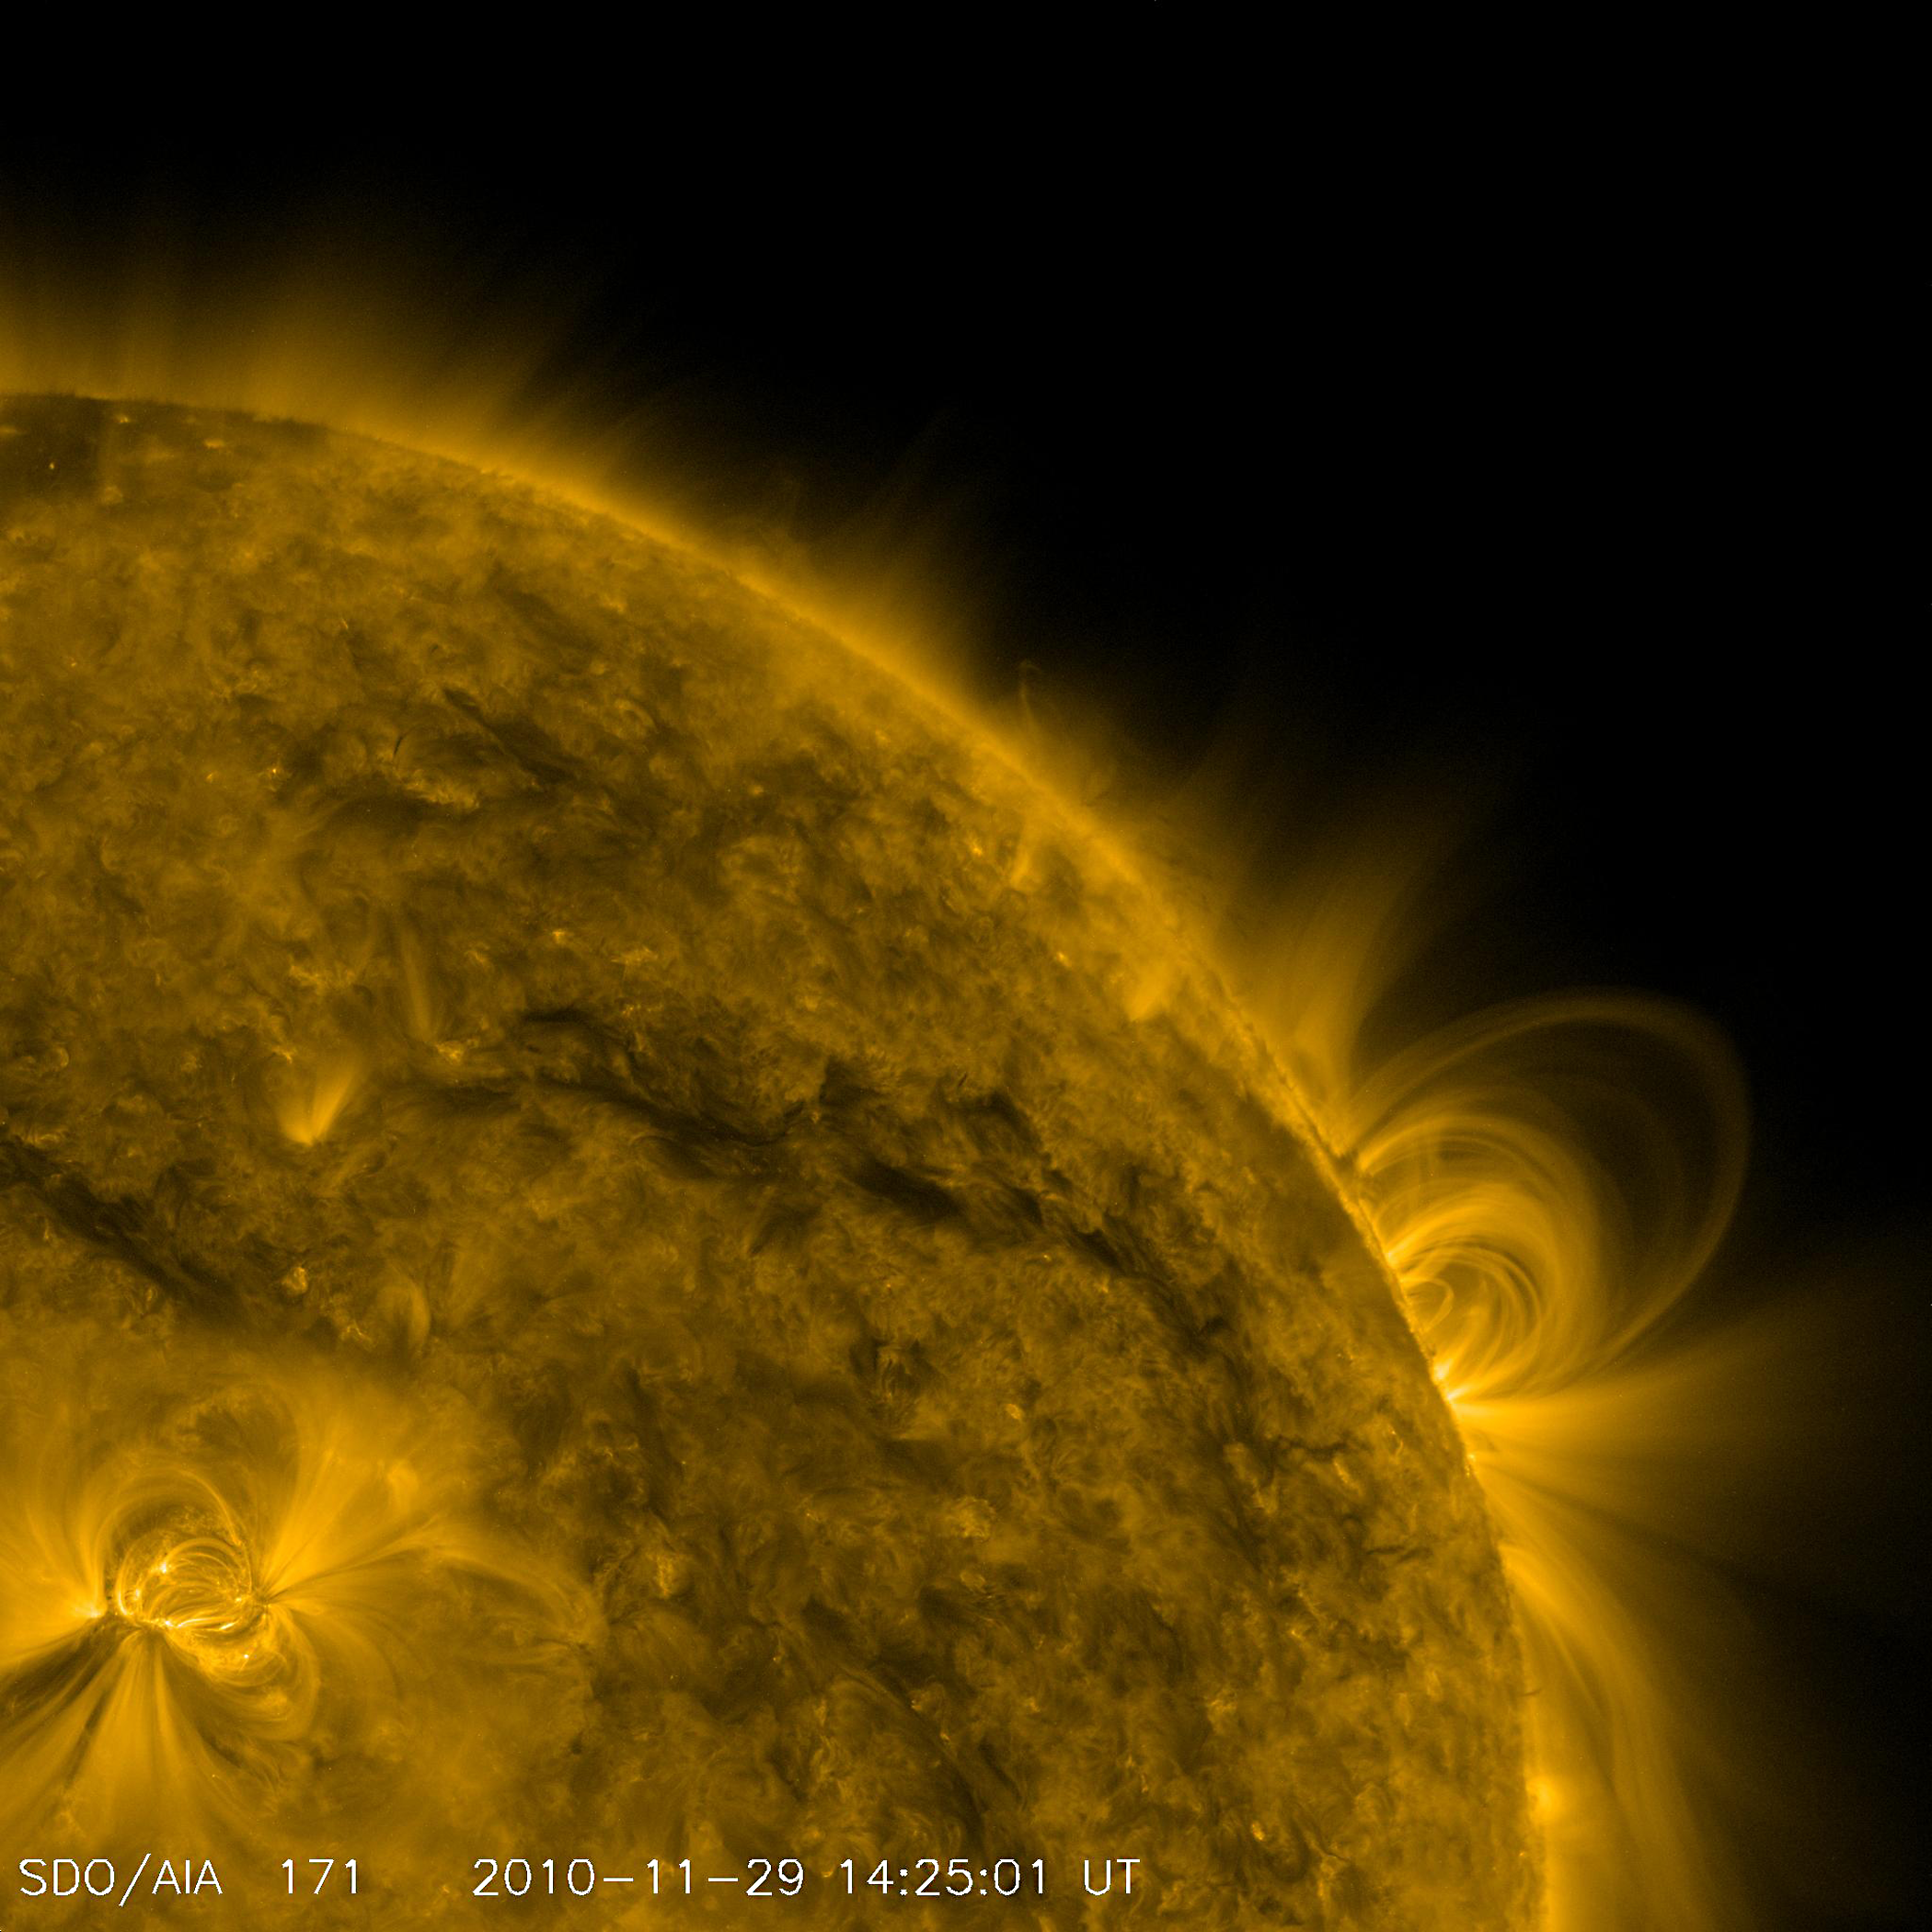
\includegraphics[width=0.6\textwidth]{figures/aia_171_loops_example.png}
	\caption{Image captured by the 171 \ang channel of the Atmospheric Imaging Assembly (AIA) onboard the Solar Dynamics Observatory (SDO). An arcade of loops in an active region can be seen on-disk in the lower left corner. Several prominent loop structures also appear off-limb on the right side. Image courtesy of NASA/SDO.}
	\label{fig:loops_example}
\end{figure}
%
\par Coronal loops, because of their relatively high temperatures ($\sim10^5-10^7$ K), are observed primarily in the extreme ultraviolet (EUV) and x-ray bands, with an associated wavelength range of $1\sim100$ \ang. While most coronal loop temperatures exceed $10^5$ K, loop plasma can span a range of temperatures and densities, due to both the complexity of the underlying field and the fact that individual loops are thermally isolated. As a result, loops are often categorized based on their thermal properties: \textit{cool}, 0.1-1 MK, \textit{warm}, 1-1.5 MK, and \textit{hot}, $\ge2$ MK \citep{reale_coronal_2010}. Whether these thermal categories actually represent distinct classes of loops or if they are all just transient states of the same type of loop is an open question in the coronal loops community, with the main debate revolving around whether different physical processes are at work in each type of loop. Additionally, loops have also been observed in several topologically different features on the Sun. See Table \ref{tab:loop_params} for some typical parameters associated with these distinct regions. This work will focus primarily on simulating loops in active regions, where many hot, nonflaring loops have been observed and emission from loop plasma is unlikely to be contaminated by radiation from the underlying transition region \citep{tripathi_emission_2011,warren_constraints_2011,warren_systematic_2012,winebarger_using_2011}. 
%\par Unfortunately, observational measurements of the coronal magnetic field are difficult and often involve a number of restrictive assumptions regarding the field topology and dynamics. Solar magnetograms can be constructed from measurements of the photospheric field through the effect of Zeeman splitting on spectral lines. The coronal field is then extrapolated, using the magnetogram as a lower boundary condition \citep[see][Ch. 5]{aschwanden_physics_2006}.
%
\begin{table}[htb]
	\centering
	\caption{Typical parameters for several different types of loops. Adapted from \citet{reale_coronal_2010}.\label{tab:loop_params}}
	\begin{tabular}{l | c c c}
		\hline\hline
		Region & $L$ [$10^9$ cm] & $T$ [$10^6$ K] & $n$ [$10^9$ cm$^{-3}$] \\
		\hline
		Bright points & 0.1-1 & 2 & 5 \\
		Active regions & 1-10 & 3 & 1-10 \\
		Giant arches & 10-100 & 1-2 & 0.1-1 \\
		Flaring loops & 1-10 & $>10$ & $>50$ \\
		\hline
	\end{tabular}
\end{table}
%
\section{Observations}
\label{sec:observations}
\hl{Discuss some observations of loops and what has been learned about them, what constraints, multi-stranded versus single stranded
Show some pretty pictures; if coronal loops are heated by nanoflares, what would be the observational signature?}
%
\par The first evidence of magnetically confined loop structures came from soft x-ray observations by grazing-incidence telescopes aboard rocket missions in the late 1960s as reported by \citet{vaiana_x-ray_1968}. Analysis of data from these early missions also allowed for classification of distinct topological features on the solar surface by \citet{vaiana_identification_1973} (see Table \ref{tab:loop_params}). These early findings provided the first look at the x-ray-bright, highly-structured corona; however, the short observing times of these rocket missions prevented systematic studies of these newly-discovered structures. The first sustained coronal loop observations did not come until the Orbiting Solar Observatory IV, equipped with a grazing-incidence x-ray telescope, and the x-ray telescope aboard the \textit{Skylab} space station \citep{krieger_results_1972,reale_coronal_2010}. Long observing times allowed for more accurate determinations of loop lifetimes, better comparisons between observations and loop models, and, perhaps most importantly, the finding that the coronal loop is the essential building block of all coronal structures \citep{rosner_dynamics_1978}. 
%
\par \hl{Need to introduce heating properties, frequency as the parameter we are most concerned about, review arguments for steady versus impulsive heating}
%
\par In order to make accurate determinations regarding the physical processes and properties of coronal loops, large statistical surveys are needed. However, isolating and analyzing individual loops is incredibly difficult, due primarily to inadequate instrument resolution relative to coronal length scales. In general, loop structures resolved by current observing instruments are considered to be \textit{multi-stranded}; that is, they are composed of many sub-resolution \textit{strands}, where a strand is the smallest loop for which the cross-section is isothermal \citep{bradshaw_diagnosing_2012}. 
%
\hl{Need something here about active region cores specifically and why we choose to study these over other parts of the AR}
%
\section{Modeling}
\label{sec:modeling}
%
\hl{Discuss modeling approaches, hydrodynamics versus magnetohydrodynamics, etc.}
\subsection{Static versus Dynamic}
\label{subsec:static_v_dynamic}
%
\hl{arguments for both; hydrostatic solutions briefly; scaling laws}
\hl{maybe combine MHD and hydrodynamics into single section, briefly mentioning MHD and why we discard the field}
\subsection{Magnetohydrodynamics}
\label{subsec:mhd}
%
\subsection{Hydrodynamics}
\label{subsec:hydro}
%
%
%?\subsection{Kinetic Modeling}
\section{Summary}

\chapter{Emission Diagnostics}
\label{ch:emission}
\hl{This chapter will discuss emission measure (EM), differential EM (DEM), line intensities etc.
and how they are interpreted in observational and modeling contexts
Discuss how this is how we know anything about plasma in the solar atmosphere
Can discuss forward modeling as well; this sets us up for the rest of the thesis}
%
\par In solar physics (and astrophysics in general), all observational data must be collected through \textit{remote sensing} techniques rather than \textit{in situ} measurements due to the great distances and extreme environments inherent to the discipline. This means that atomic data and spectroscopy must be used to infer properties about the coronal plasma, including the temperature and density. To a good approximation, the hot, tenuous coronal plasma is \textit{optically thin} to radiation emitted in the visible, ultraviolet (UV), and x-ray bands. This means that, between the observer and where the radiation was produced, the photons were not scattered or absorbed and reemitted. As a result, the observed radiation contains signatures of the plasma that produced it and has not been polluted by some intermediate process.
%
\section{Spectral Line Intensity}
\label{sec:spectral_lines}
%
As discussed in \S\ref{sec:coronal_heating}, spectroscopy has been a critically important tool in solar physics since the discovery of the million-degree corona. Modern observing instruments and techniques have allowed for the collection of an unprecedented amount of data at increasingly higher spatial resolution and temporal cadence. However, interpreting this spectroscopic data in terms of useful plasma parameters (e.g. density and temperature) continues to pose a challenge to both observers and modelers alike.
%
\par The dominant emission mechanism in the high-temperature, low-density solar corona is \textit{bound-bound} emission,
\begin{equation}
	\label{eq:bound_bound}
	X_j^{+m}\to X_i^{+m} + h\nu_{j,i},
\end{equation}
where $X$ represents the atomic species, $m$ is the charge state, $h$ is Planck's constant, and $\nu_{j,i}$ is the frequency of the emitted photon of energy $\Delta E_{j,i} = h\nu_{j,i}=hc/\lambda_{j,i}$, with $j$ and $i$ representing the bound and lower energy states, respectively \citep{mason_spectroscopic_1994}. In this process, ion $X^{+m}$ spontaneously decays from excited state $j$ to lower-energy state $i$, emitting a photon of frequency $\Delta E_{j,i}$. The associated emissivity (power per unit volume) for the transition can then be written as 
\begin{equation}
	\label{eq:emissivity}
	P(\lambda_{j,i})=N_j(X^{+m})A_{j,i}\Delta E_{j,i},
\end{equation}
where $N_j(X^{+m})$ is the number density of element $X$ with charge state $+m$ in excited state $j$ and $A_{j,i}$ is the Einstein spontaneous emission coefficient. Thus, the power for a given spectral line is dependent on both the number of ions of a particular charge state and the number of ions in that particular charge state who are also in an excited state \citep{mason_spectroscopic_1994,bradshaw_collisional_2013}. Finally, this volumetric power can be related to the observed line intensity as at Earth,
\begin{equation}
	\label{eq:intensity}
	I(\lambda_{j,i}) = \frac{1}{4\pi R^2}\int_V \mathrm{d}V~P(\lambda_{j,i}),
\end{equation}
where the integral is taken over the entire sphere of radius $R$, where $R$ is the distance to the observer, and then normalized by the surface area of the sphere.
%
\par The next question is of course how these measured line intensities can be related to the properties of the coronal plasma. In Eq. \ref{eq:emissivity}, $A_{j,i}$ can be calculated from laboratory experiments for a given transition and $\Delta E_{j,i}$ is easily found provided $\lambda_{j,i}$ is known. The remaining quantity, $N_j(X^{+m})$ can be expressed as a series of ratios,
\begin{equation}
	\label{eq:density_jm}
	N_j(X^{+m})=\frac{N_j(X^{+m})}{N(X^{+m})}\frac{N(X^{+m})}{N(X)}\frac{N(X)}{N(H)}\frac{N(H)}{N_e}N_e,
\end{equation}
where $N(X^{+m})$ is the number density of element $X$ in charge state $+m$, $N(X)$ is the number density of element $X$, $N(H)$ is the number density of hydrogen, and $N_e$ is the electron number density \citep{mason_spectroscopic_1994}. Note that $N_j(X^{+m})$ has just been repeatedly multiplied by one in order to reexpress it in terms of the following ratios (from left to right in Eq. \ref{eq:density_jm}): fraction of $+m$-ions in excited state $j$, fraction of $X$ atoms in charge state $+m$, relative abundance of $X$ compared to hydrogen, and relative abundance of hydrogen compared to the number of electrons. The expression can be further simplified through the definition of the relative abundance $\mathrm{Ab}_X=N(X)/N(H)$ and the common approximation $N(H)/N_e\approx0.83$.
%
\par Eq. \ref{eq:emissivity}, and thus Eq. \ref{eq:intensity}, can be further simplified by invoking the \textit{coronal model} approximation. In optically-thin plasmas, it can be assumed that the collisional excitation and radiative decay occur from and to the ground state, respectively; in other words $i\to g$, with g representing the ground state. Additionally, the processes which determine the excitation level and those that determine the charge state are assumed to operate on disparate enough timescales such that the changes in energy level populations of the emitting ions, occurring on short timescales, can be decoupled from the changes in the charge state, occurring on longer timescales \citep{bradshaw_collisional_2013}. Using these assumptions, statistical equilibrium between the spontaneous decay and collisional excitation processes demands
\begin{equation}
	\label{eq:stat_eq}
	N_g(X^{+m})N_eC^e_{g,j} = N_j(X^{+m})A_{j,g},
\end{equation}
where $C^e_{g,j}$ is the electron collisional excitation rate between $g$ and $j$ \citep{bradshaw_collisional_2013}. Plugging Eqs. \ref{eq:stat_eq} and \ref{eq:density_jm} into Eq. \ref{eq:emissivity} and letting $N_g(X^{+m})\approx N(X^{+m})$ yields
\begin{equation}
	\label{eq:emissivity_simple}
	P(\lambda_{j,g})=(0.83)\mathrm{Ab}_X\Delta E_{j,g}\frac{N(X^{+m})}{N(X)}C^e_{j,g}N_e^2.
\end{equation}
Defining the \textit{contribution function} $G(T,\lambda_{j,g})=N(X^{+m})/N(X)C^e_{j,g}$, the intensity integral can be rewritten as
\begin{equation}
	I(\lambda_{j,g}) = \frac{(0.83)\mathrm{Ab}_X\Delta E_{j,g}}{4\pi R^2}\int_V\mathrm{d}V~N_e^2G(T,\lambda_{j,g}).
\end{equation}
If the plasma is isothermal over the emitting volume $V$, $G(T,\lambda_{j,g})$ comes outside the integral such that 
\begin{equation}
	\label{eq:intensity_isothermal}
	I(\lambda_{j,g}) = \frac{(0.83)\mathrm{Ab}_X\Delta E_{j,g}}{4\pi R^2}G(T,\lambda_{j,g})\langle\mathrm{EM}\rangle,
\end{equation}
where $\langle\mathrm{EM}\rangle=\int_V\mathrm{d}V~N_e^2$ is the average \textit{emission measure}. However, in many cases, this isothermal approximation does not hold such that the intensity integral must be expressed as 
\begin{equation}
	\label{eq:dem_integral}
	I(\lambda_{j,g}) = \frac{(0.83)\mathrm{Ab}_X\Delta E_{j,g}}{4\pi R^2}\int_V\mathrm{d}T~\phi(T)G(T,\lambda_{j,g}),
\end{equation}
where $\phi(T)=N_e^2\mathrm{d}V/\mathrm{d}T$ is the \textit{differential emission measure} ($\mathrm{DEM}$). 
%%
\section{Differential Emission Measure}
\label{sec:dem}
%
\par The $\mathrm{DEM}$ and $\mathrm{EM}$ provide information about the temperature distribution of the plasma. In particular, the $\mathrm{DEM}$ is a measure of the amount of emitting material at a particular temperature $T$ in the plasma. Thus, the $\mathrm{DEM}$ is an observable that any viable theory of coronal heating should be able to predict with reasonable accuracy \citep{golub_solar_2010}. Furthermore, because the $\mathrm{DEM}$ is a one-dimensional function, it provides a simple and powerful characterization of the multi-thermal coronal plasma. Unfortunately, calculating these quantities from observed line intensities is difficult because of both mathematical and data availability issues. Looking back to Eq. \ref{eq:intensity_isothermal}, one can see that, provided the line intensities and contribution functions are available over a significant range of temperatures, the emission measure can be calculated algebraically.
%
\par 
%
\begin{figure}
	\centering
	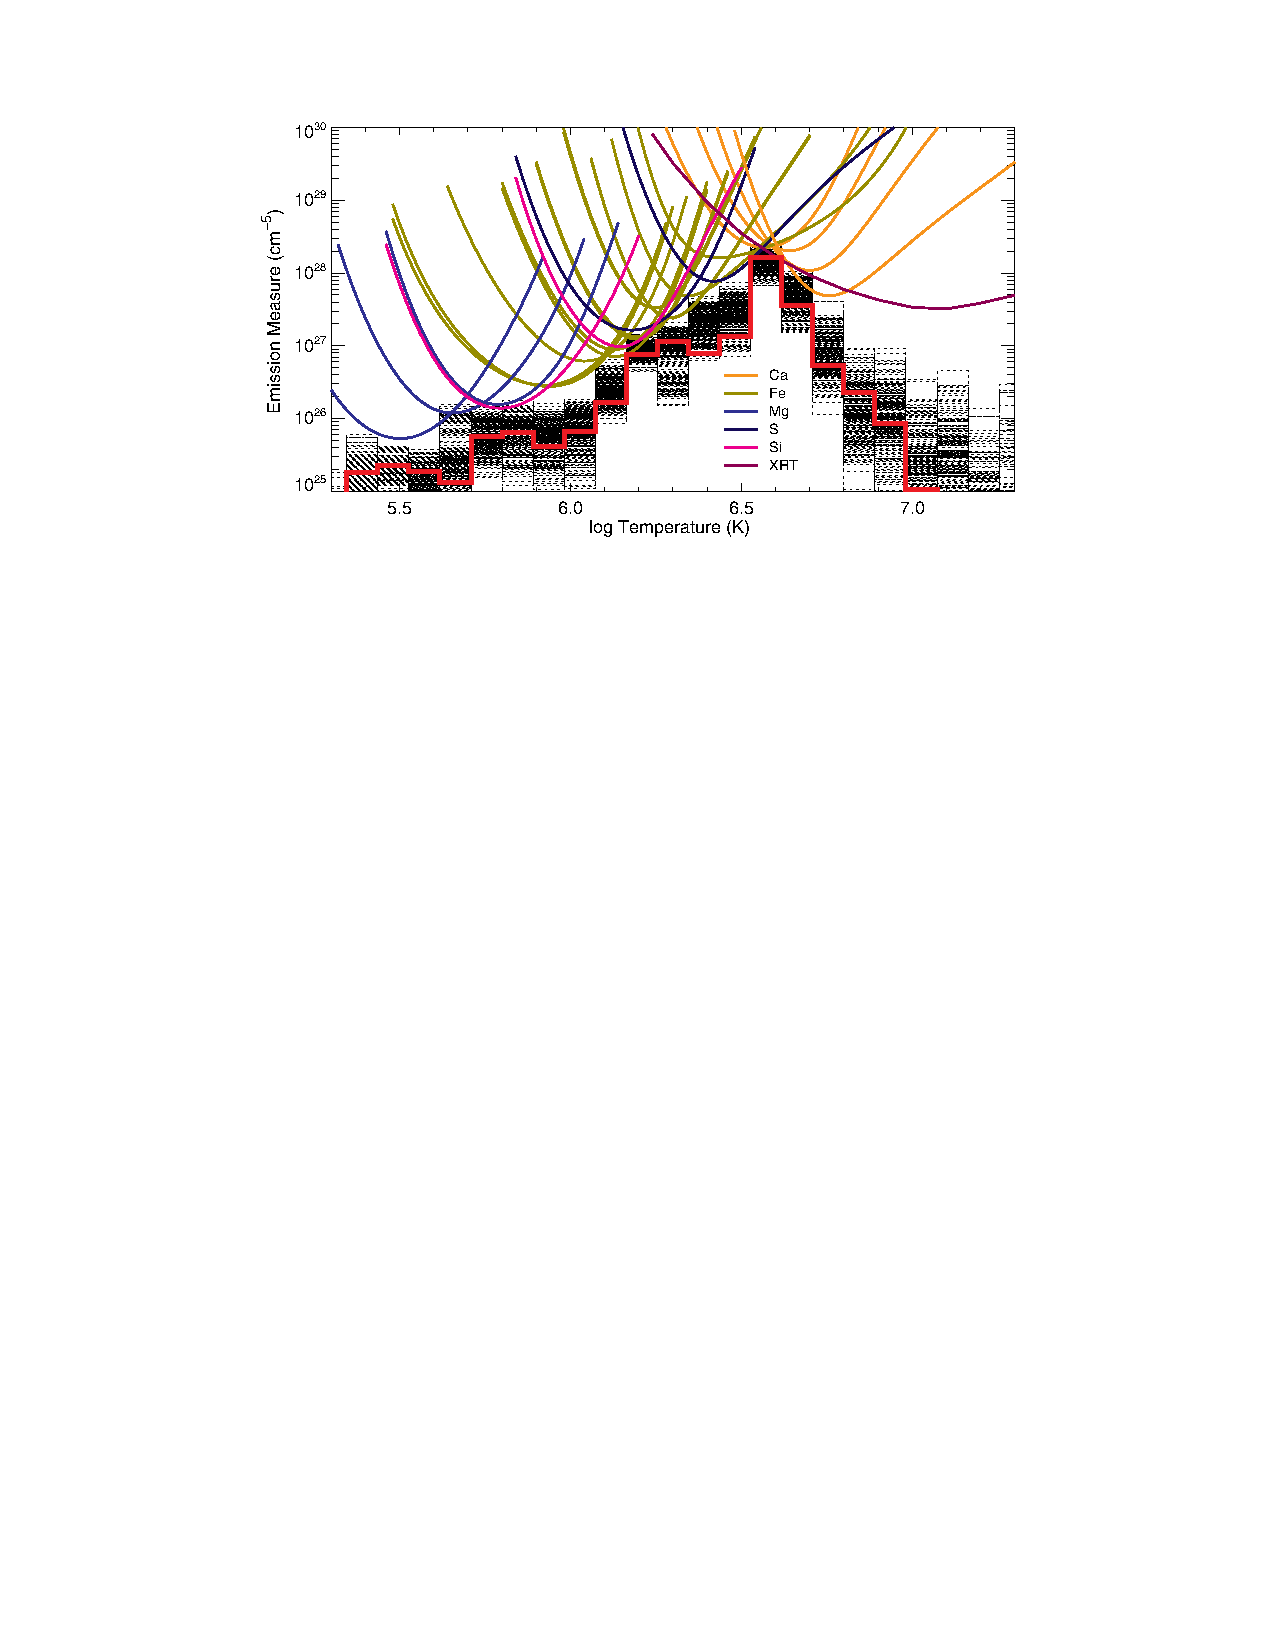
\includegraphics[width=0.75\textwidth]{figures/dem_em_loci.pdf}
	\caption{Emission measure distribution reconstruction for an active region core. The colored curves show the emission measure calculation using the $\mathrm{EM}$ loci method. The black and red histograms show the $\mathrm{DEM}(T)\mathrm{d}T$ reconstructed using the MCMC method of \citet{kashyap_markov-chain_1998}. Here, the $\mathrm{DEM}$ is multiplied by the temperature bin for comparison with the $\mathrm{EM}$ loci calculation. Image taken from \citet{warren_constraints_2011}}
	\label{fig:dem_em_loci}
\end{figure}
%
\par Unlike $\langle\mathrm{EM}\rangle$, $\phi(T)$ cannot be determined algebraically; instead, Eq. \ref{eq:dem_integral}, a Fredholm equation of the first kind, must be inverted to find $\phi(T)$, a task that poses well-known mathematical difficulties \citep{kashyap_markov-chain_1998}. One method for performing such an inversion is a discretization of Eq. \ref{eq:dem_integral}
\begin{equation}
	\label{eq:disc_dem_integral}
	I_j = \frac{(0.83)\mathrm{Ab}_X\Delta E_j}{4\pi R^2}\sum_{k=1}^N\phi_k\int^{T_{k+1}}_{T_k}\mathrm{d}T~G_j(T),
\end{equation}
where $j$ labels the spectral line and $[T_{k+1},T_k]$ is the temperature interval over which $\phi_k$ is constant. For each measured line intensity $I_j$, $\phi_k$ for $1\le k\le N$ are determined through some minimization procedure \citep{landi_monte_2012}. To calculate the $\mathrm{DEM}$ curve, an arbitrary spline or polynomial is first assumed; subsequent corrections at $T_{eff,j}$, the temperature of maximum abundance for the line intensity $I_j$, are then calculated and a spline interpolation applied to these corrections for the entire temperature range $[T_1,T_N]$. This correction is then applied to initial curve and the corrected curve is used as the initial $\mathrm{DEM}$ on the next iteration \citep{landi_monte_2012}. This method of course has the disadvantage that a functional form for the $\mathrm{DEM}$ must be chosen \textit{a priori}, biasing the temperature distribution. Additionally, a poor choice of temperature interval in Eq. \ref{eq:disc_dem_integral} can oversmooth the $\mathrm{DEM}$ curve or cause convergence issues.
%
%\hl{Here something about emission measure scaling with temperature + observational results supporting + simulation results supporting + introduce hot emission}
\par From these emission measure distributions, simple observables can be calculated that any viable heating model should be able to produce. The most popular of these observables is the well-known scaling between the emission measure and the temperature, 
\begin{equation}
	\mathrm{EM}\propto T^a.
\end{equation}
This scaling, first proposed by \citet{jordan_energy_1980}, has since been validated by both simulation and observation. A summary of model and observational results for the $a$ parameter can be found in Table \ref{tab:em_scalings}.
%
\begin{table}
	\centering
	\caption{Summary of emission measure scalings from observational and modeling studies. Scalings are typically calculated coolward of the emission measure peak and typically range from 2 to 5. Adapted from \citet{bradshaw_diagnosing_2012}.\label{tab:em_scalings}}
	\begin{tabular}{L{4cm} l l l}
		\hline\hline
		Slopes, $a$ & Range of $\log{T}$ & Type & Reference \\
		\hline
		3.26 & 6.00-6.60 & observation & \citet{warren_constraints_2011} \\
		2.17 &  & model & \\
		\hline
		3.20 & 6.00-6.50 & observation & \citet{winebarger_using_2011} \\
		\hline
		2.08-2.47 \\ (background) & 5.50-6.55 & observation & \citet{tripathi_emission_2011} \\
		2.05-2.70 \\ (background subtracted) &  &  & \\
		\hline
		1.60-2.00 \\ (photospheric abundances) & 6.00-[6.60-6.80] & model & \citet{mulu-moore_can_2011} \\
		2.00-2.30 \\ (coronal abundances) &  &  & \\
		\hline
		1.70-4.50 & 6.00-6.60 & observation & \citet{warren_systematic_2012} \\ 
		\hline
		1.91-5.17 & 6.00-[6.30,6.80] & observation & \citet{schmelz_cold_2012} \\
		\hline
		0.58-2.24 \\ (low-frequency nanoflares) & 6.00-$\log{T_{peak}}$ & model & \citet{bradshaw_diagnosing_2012} \\
		\hline
		0.79-3.65 \\ (nanoflare trains) & 6.00-$\log{T_{peak}}$ & model & \citet{reep_diagnosing_2013} \\
		\hline
		$\sim2-\sim7$ \\ (low- to high-frequency heating) & [6.00-6.25]-$\log{T_{peak}}$ & model & \citet{cargill_active_2014} \\
		\hline
	\end{tabular}
\end{table}
%%
\section{Plasma Charge State: Equilibrium and Non-equilibrium}
\label{sec:charge_state}
%
\par \hl{Talk about forward modeling procedure, why it is important, how it is done, CHIANTI, hydrodynamics, some nice pictures}
%
%%
\chapter{Numerical Modeling}
\label{ch:numerical}
%
\par Coronal loop modeling can be roughly divided into two categories: multi-dimensional (typically 3D) magnetohydrodynamic models and hydrodynamic models. The former focuses primarily on the study of the dynamics of the magnetic field itself; the latter concentrates on the response of the plasma for some \textit{ad-hoc} heating and prescribed, static field geometry \citep{bradshaw_influence_2013}. While a hydrodynamic treatment may seem overly simplified, such models often provide a much more physically realizable treatment of the plasma than most 3D MHD models. This thesis will examine primarily the use of hydrodynamic models in the study of coronal plasma dynamics. By using hydrodynamic models, the evolution and response of the plasma to various heating functions can be carefully treated. In particular, this work will focus on the role of a two-fluid treatment in efficient hydrodynamic simulations. Such efficient models allow for the exploration of large parameter spaces with comparably little computational overhead.
%
\section{One-dimensional Two-fluid Hydrodynamics}
\label{sec:1dhydro}
%
\par In \S\ref{subsec:hydro}, the hydrodynamic equations were discussed under the assumption that the electron and ion populations were in equilibrium at all times (i.e. a single-fluid approximation). However, since the mechanism behind coronal heating is still highly debated, the degree to which the ions or electrons are preferentially heated is unknown. It is often assumed that the electrons are the direct recipients of the prescribed heating function. However, it is also possible that the ions are preferentially heated. One particular example is that of ion-cyclotron wave resonances \citep{markovskii_intermittent_2004}. Ion cyclotron waves are excited by plasma instabilities in the lower corona. These waves then propagate upwards through the coronal plasma and wave particle interactions can occur for those ions whose gyrofrequencies have a resonance with the ion-cyclotron wave. Additionally, there is also evidence for ion heating via reconnection, both in laboratory plasmas and particle-in-cell simulations \citep{ono_ion_1996,yoo_bulk_2014,drake_onset_2014}. Thus, ion heating in the solar corona should not be discounted as a possibility.
%
\par In this work, quasi-neutrality, $n_e=n_i=n$, will be assumed. While the heavier ions are in higher charge states and have thus given up more than one electron per ion, $\mathrm{Ab}_{\mathrm{H}}\gg\mathrm{Ab}_{X>\mathrm{H}}$. In other words, the abundance of (singly ionized) H is so much greater than the multiply-ionized heavier elements that quasi-neutrality is a valid assumption. Additionally, current-free conditions are also assumed such that $v_e=v_i=v$. Under these assumptions, the conservative forms of the mass and momentum equations can be written,
\begin{align}
	\frac{\partial\rho}{\partial t} &= -\frac{\partial(\rho v)}{\partial s} \label{eq:1dmass}, \\[0.5em]
	\frac{\partial(\rho v)}{\partial t} &= -\frac{\partial(\rho v^2)}{\partial s}-\frac{\partial(p_e + p_i)}{\partial s} + \frac{\partial}{\partial s}\left(\frac{4}{3}\mu_i\frac{\partial v}{\partial s}\right) + \rho g_{\parallel}, \label{eq:1dmom}
\end{align}
where $\rho=m_en_e + m_in_i=n(m_e+m_i)\approx nm_i$, $m_i$ is the ion mass, $p_e$ and $p_i$ are the electron and ion pressures respectively, and $\mu_i=m_iu_i$, where $u_i$ is the classical Spitzer viscosity coefficient \citep{bradshaw_influence_2013}. Notice that Eq. \ref{eq:1dmass} is equivalent to its single-fluid counterpart due to our assumption of quasi-neutrality and that the only difference between Eq. \ref{eq:1dmom} and Eq. \hl{SF MOM EQ REF HERE} is the addition of the ion viscosity term and that $p=p_e+p_i$.
%
\par The electron and ion energy equations are given by
\begin{align}
	\frac{\partial E_e}{\partial t} &= -\frac{\partial}{\partial s} \lbrack(E_e+p_e)v\rbrack+v\frac{\partial p_e}{\partial s} - \frac{\partial F_{e}}{\partial s} + \frac{1}{\gamma - 1}k_Bn\nu_{ei}(T_i-T_e) -E_R+E_{H,e}, \label{eq:1denergy_e} \\[0.5em]
	\frac{\partial E_i}{\partial t} &= -\frac{\partial }{\partial s}\lbrack(E_i+p_i)v\rbrack-v\frac{\partial p_e}{\partial s} - \frac{\partial F_{i}}{\partial s} + \frac{1}{\gamma - 1}k_Bn\nu_{ei}(T_e-T_i) + \frac{\partial}{\partial s}\left(\frac{4}{3}\mu_iv\frac{\partial v}{\partial s}\right) +\rho v g_{\parallel} + E_{H,i},\label{eq:1denergy_i}
\end{align}
where $E_e$ and $E_i$ are the electron and ion energies, respectively, and $E_{H,e}$ and $E_{H,i}$ are the \textit{ad-hoc} volumetric heating rates for the electrons and ions, respectively. Furthermore, this set of equations is subject to the closure conditions
\begin{align}
	E_e = \frac{p_e}{\gamma - 1}, \label{eq:ee_close} \\[0.5em]
	E_i = \frac{p_i}{\gamma - 1} + \frac{1}{2}\rho v^2, \label{eq:ei_close} \\[0.5em]
	p_e = k_BnT_e, \label{eq:pe_close} \\[0.5em]
	p_i = k_BnT_i, \label{eq:pi_close}
\end{align}
where $\gamma=5/3$ is the adiabatic index.
% 
\par The conductive heat fluxes for the ions and electrons, $F_{e}$ and $F_{i}$, are given by the classical Spitzer-Harm \citep{spitzer_transport_1953} formulas
\begin{align}
	F_{e}=-\kappa_{0,e}T_e^{5/2}\frac{\partial T_e}{\partial s}, \label{eq:1dhfluxe} \\[0.5em]
	F_{i}=-\kappa_{0,i}T_i^{5/2}\frac{\partial T_i}{\partial s}, \label{eq:1dhfluxi}
\end{align}
where $\kappa_{0,e}$ and $\kappa_{0,i}$ are the Spitzer coefficients for electron and ion thermal conduction, respectively \citep{bradshaw_influence_2013}. The classical formula for the heat flux, however, is known to be inaccurate at high temperatures and low densities. To correct for this, a flux-limiter or free-streaming limit is often used, such that the heat flux saturates at
\begin{equation}
	\label{eq:free_stream_limit}
	F_{sat,s} = -\beta\frac{3}{2}\frac{k^{3/2}}{m_s^{1/2}}nT_s^{3/2},
\end{equation}
where $s$ specifies the particles species \citep{bradshaw_explosive_2006}. This prevents the heat flux from becoming unphysically large, particularly during the onset of heating when the temperature is high and the density relatively low. $\beta$ is a flux limiter constant with a typical value between $1$ and $1/6$ \citep{luciani_nonlocal_1983,karpen_nonlocal_1987}. The final expression for the conductive flux for species $s$ can then be written as
\begin{equation}
	\label{eq:flux_limited}
	F_s=\frac{F_{c,s}F_{sat,s}}{\sqrt{F_{c,s}^2 + F_{sat,s}^2}},
\end{equation}
where $F_{c,s}$ is the classical expression for the heat flux for species $s$ as given in Eqs. \ref{eq:1dhfluxe} and \ref{eq:1dhfluxi}. Thus, $F_s\approx F_{c,s}$ when $|F_{c,s}|\ll|F_{sat,s}|$ and $F_s\approx F_{sat,s}$ when $|F_{c,s}|\gg|F_{sat,s}|$.
%
\par The electron and ion energy equations are coupled through a collisional term proportional to the Coulomb collision frequency times the difference between the temperatures of the respective species. The Coulomb collision frequency is given by
\begin{equation}
	\nu_{ei} = \frac{16\sqrt{\pi}}{3}\frac{e^4}{m_em_i}\left(\frac{2k_BT_e}{m_e}\right)^{-3/2}n\ln{\Lambda},
\end{equation}
where $\ln{\Lambda}\approx20$ is the Coulomb logarithm. If the heating timscale is much greater than $1/\nu_{ei}$, the collisional timescale, then electron-ion equilibrium cannot be assumed during the heating phase. In particular, for $n\sim10^8~\mathrm{cm}^{-3}$ and $T\sim10^7~\mathrm{K}$, parameters typical of a nanoflare-heated coronal plasma, the collisional timescale can be estimated as $\tau_{ei,coll}\sim1/\nu_{ei}\approx8000$ s. So any heating occurring on a timescale less than 8000 s will force the electron and ion populations out of equilibrium. Often when modeling nanoflares, heating timescales of a few hundreds or even a few tens of seconds are used. Thus, treating the evolution of the electron and ions separately is particularly important when studying impulsive heating in coronal loops.
%
\section{``0''-Dimensional Hydrodynamic Models }
\label{sec:0dmodels}
%
\par As discussed in \S\ref{sec:1dhydro} and \S\ref{subsec:hydro}, 1D hydrodynamic models are an invaluable tool for studying the plasma dynamics of the solar corona. However, while these models only consider evolution in the field-aligned direction, their solutions still necessitate a careful treatment of several highly-nonlinear partial differential equations. Perhaps the greatest restriction imposed on these models is the need to resolve the thermal conduction timescale, given by $\Delta t_C=4\times10^{-10}n\Delta s^2/T^{5/2}$. For a transition region plasma with an adequate grid size, this can result in a timestep on the order of several milliseconds \citep{bradshaw_influence_2013}. This makes modeling events in excess of a few hours tedious and computing thousands of field lines nearly impossible. Additionally, as 1D hydrodynamic codes become more sophisticated, incorporating features such as adaptive mesh refinement and effects due to non-equilibrium ionization, their output becomes increasingly more complicated and difficult to interpret \citep{cargill_enthalpy-based_2012-1}.
%
\par Thus, there is a need for codes which a) provide an efficient way to model dynamic coronal loops and b) generate output that provides physical insight into the evolution of the plasma and the resulting physical observables. Zero-dimensional or ``0D'' hydrodynamic models satisfy both of these requirements. 0D models have long been used as a tool to better understand static and dynamic coronal loop configurations. They provide a way to efficiently compute loop parameters such as $T$ and $n$ while incorporating the plasma processes known to be dominant in coronal loops. Most 0D loop models compute spatially-averaged time-dependent quantities and thus provide a way to perform large parameter-space surveys in reasonable amounts of time while relaxing the static equilibrium assumption.
%
\par The scaling laws of \citet{rosner_dynamics_1978} are often considered some of the first 0D models as they provided simple expressions for relating the loop length, temperature, pressure, and heating rate. However, these analytic models did not provide a way to analyze loop dynamics. In the last thirty years, several 0D models have attempted to provide efficient ways to model loop dynamics. These include, but are not limited to, \citet{fisher_equation_1990,kopp_coronal_1993,cargill_implications_1994,aschwanden_hydrodynamic_2009}. While many of these 0D models provided good insight into different regimes of loop evolution, \citet{cargill_enthalpy-based_2012-1} show that each of these approaches has significant drawbacks when one considers the evolution of the loop throughout an entire cycle of heating and cooling. In particular, many do not treat the conductive and radiative cooling regimes correctly, do not allow for a generalized heating function, and/or do not carefully take into account the coupling between the corona and transition region. 
%
%
\subsection{The EBTEL Model}
\label{subsec:ebtel}
%
\par The Enthalpy-Based Thermal Evolution of Loops (EBTEL) model \citep{klimchuk_highly_2008,cargill_enthalpy-based_2012} was developed initially to study nanoflare heating, but can handle a generalized heating input. EBTEL divides the loop into coronal and transition region parts, where the boundary is defined by the location at which thermal conduction switches from a source term (transition region) to a loss term (corona). The basic idea behind EBTEL, as the name implies, is to equate an enthalpy flux with any difference in magnitude between the conductive heat flux and the radiative losses from the transition region \citep{klimchuk_highly_2008}. In this way, the processes of evaporation and condensation, the filling and draining of the coronal portion of the loop, can be accurately modeled in a 0D context. 
%
\par The governing equations of the EBTEL model are derived by computing spatial averages over the coronal and transition region portions of the loop. In particular, spatial integrals of the 1D hydrostatic equations (see \S\ref{subsec:hydro}) are taken over the corona (length $L$) and the much thinner transition region (length $\ell\ll L$). EBTEL relies on several key assumptions: a) the flow is assumed to be subsonic, $v<C_s$, such that terms $\mathcal{O}(v^2)$ are ignored; b) the loop is shorter than a gravitational scale height such that gravitational terms are ignored; c) the ratios $c_2=\bar{T}/T_a$ and $c_3=T_0/T_a$, where $\bar{T},T_a,T_0$ are the coronally averaged, apex, and base temperatures, respectively, are fixed such that $c_2=0.9$ and $c_3=0.6$. Additionally, as is common in loop models, only one half of the loop is computed, with symmetry about the apex assumed \citep{klimchuk_highly_2008}.
%
\begin{figure}
	\centering
	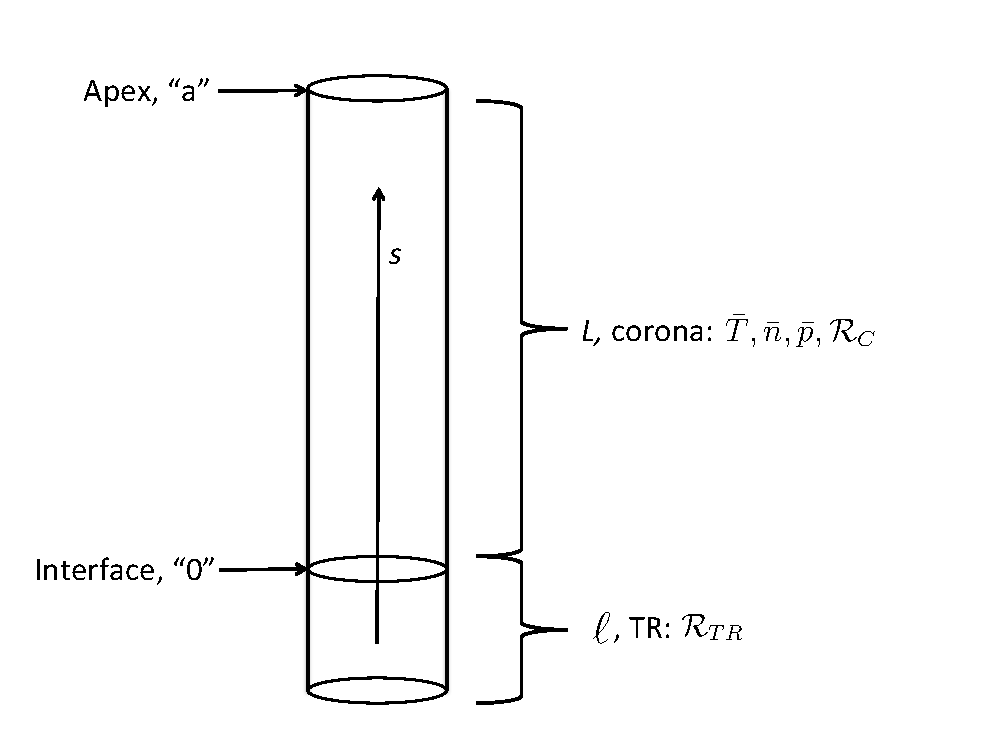
\includegraphics[width=0.6\textwidth]{figures/ebtel_schematic.pdf}
	\caption{Schematic showing how a loop half-length, with coronal portion of length $L$ and TR length $\ell$, is represented in EBTEL. Note that the loop is shown as a cylinder since (nearly) all effects due to gravitational stratification are ignored. Quantities denoted with a ``0'' subscript are evaluated at the corona-TR interface; quantities denoted with an ``a'' subscript are evaluated at the loop apex. Note that the relative size of the TR is exaggerated for the purposes of illustration and in reality $\ell\ll L$.}
	\label{fig:ebtel_schematic}
\end{figure}
%
\par The 0D EBTEL equations, as given by \citet{cargill_enthalpy-based_2012}, are
\begin{align}
	\frac{1}{\gamma - 1}\frac{d\bar{p}}{dt} = \bar{E_H} - \frac{\mathcal{R}_C}{L}(1+c_1), \label{eq:ebtel_sf_pressure} \\[0.5em]
	\frac{d\bar{n}}{dt} = -\frac{c_2(\gamma - 1)}{c_32k_B\bar{T}L\gamma}(F_0 + c_1\mathcal{R}_C), \label{eq:ebtel_sf_density}
\end{align}
where an overbar indicates the quantity is spatially averaged over the corona, $F_0$ is the heat flux at the base of the corona, $\mathcal{R}_C=\int_C\mathrm{d}s~E_R$ is the coronal spatial integral over the radiative loss term and $c_1=\mathcal{R}_{tr}/\mathcal{R}_c$ is the ratio between the spatially integrated radiative losses over the transition region and corona, respectively. Fig. \ref{fig:ebtel_schematic} shows the EBTEL geometry and the quantities associated with each region. The main advantage EBTEL has over other 0D codes is its treatement of the interaction between the corona and transition region. Additionally, Eqs. \ref{eq:ebtel_sf_pressure} and \ref{eq:ebtel_sf_density} are closed by an equation of state, $\bar{p}=2\bar{n}k_B\bar{T}$, such that, given $\bar{n}$ and $\bar{p}$, the temperature $\bar{T}$ can be determined. It should be noted that \citet{klimchuk_highly_2008} determined that $c_1=4.0$ through an empirical method based on 1D hydrodynamic simulations. \citet{cargill_enthalpy-based_2012} later improved on this assumption by adding corrections for gravity and an improved estimated during the radiative cooling phase.
%
\begin{figure}
	\centering
	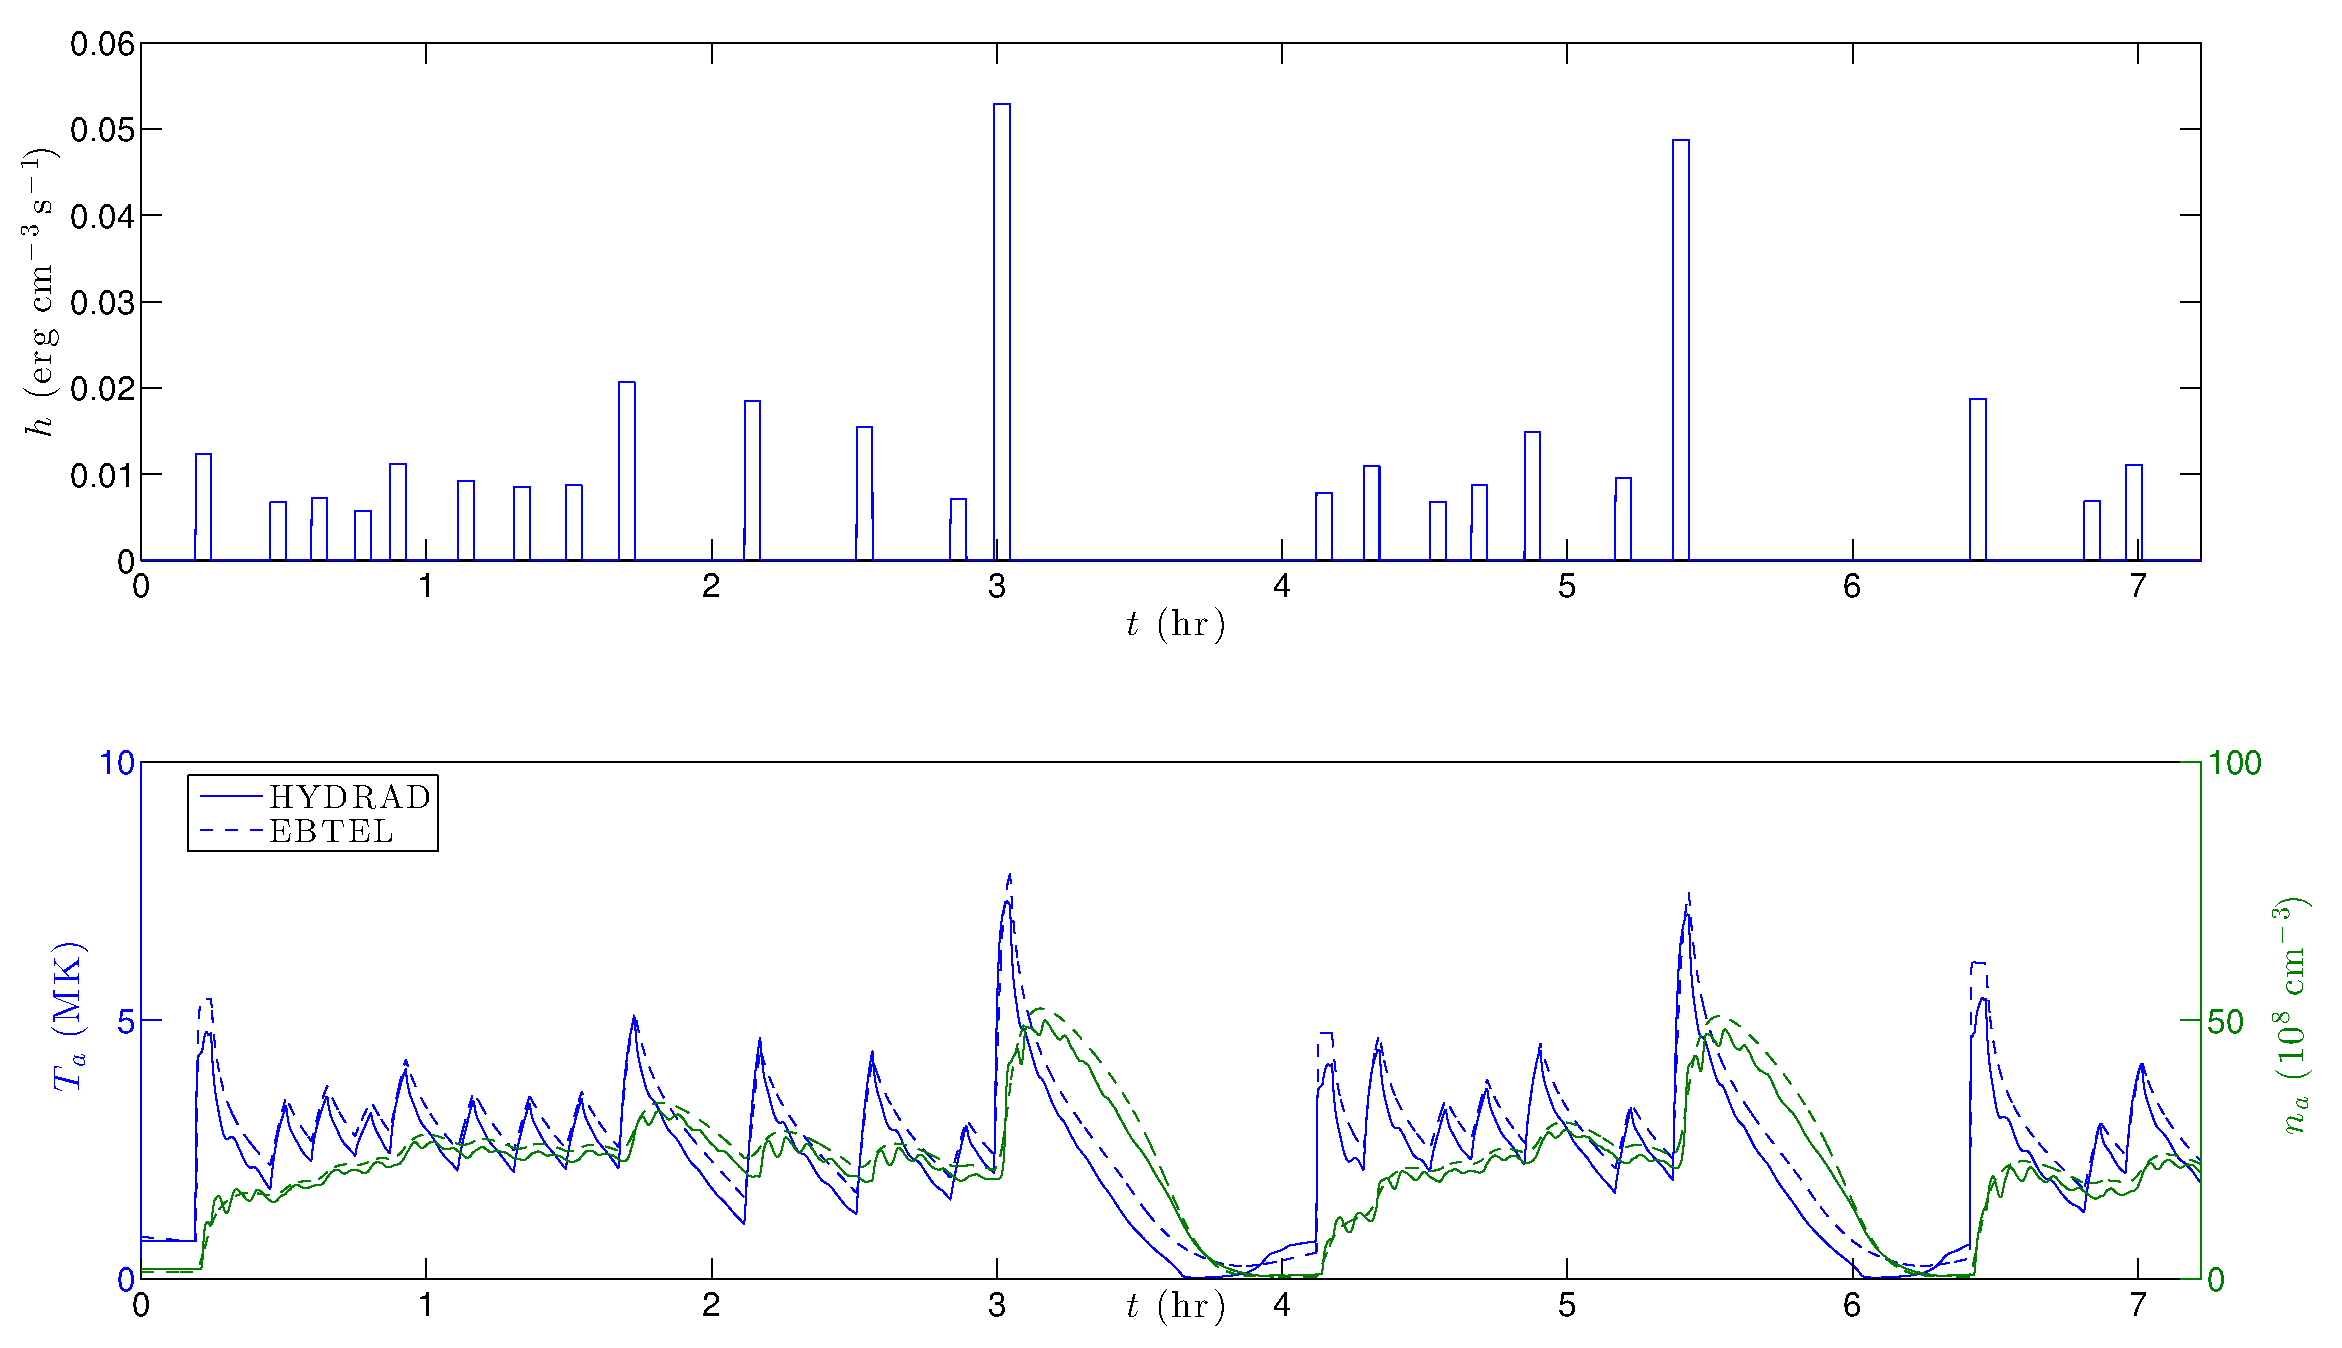
\includegraphics[width=0.95\textwidth]{figures/ebtel_sf_compare.eps}
	\caption{Comparison between EBTEL (dashed) and the 1D hydrodynamic code HYDRAD (solid) for a heating function with randomly chosen start times and amplitudes chosen from a power-law distribution. The upper panel shows the heating profile, the middle panel shows the temperature profiles, and the bottom panel shows the density profiles.For both the temperature and density, the EBTEL profile follows the HYDRAD profile quite closely. For the EBTEL profiles, the apex quantities are shown here. For the HYDRAD profiles, the quantities are averaged over the upper portion of the loop.}
	\label{fig:ebtel_sf_compare}
\end{figure}
%
\par EBTEL has been carefully benchmarked with the 1D hydrodynamic code HYDRAD. Fig. \ref{fig:ebtel_sf_compare} shows a comparison between EBTEL and HYDRAD for a series of impulsive, square heating events whose amplitudes are chosen from a power-law distribution. \citet{cargill_enthalpy-based_2012} also provide several comparisons between EBTEL and HYDRAD for triangluar, square, and gaussian heating pulses of varying duration and amplitude. Additionally, \citet{cargill_enthalpy-based_2012-1} show comparisons between EBTEL, HYDRAD, and earlier 0D models in an effort to show how EBTEL improves upon previous 0D efforts by matching 1D codes in both the initial heating and subsequent cooling phases of loop evolution.
%
\par Since its initial introduction by \citet{klimchuk_highly_2008}, EBTEL has been used successfully in a large number of published studies by both modelers and observers alike. For example, \citet{ugarte-urra_determining_2014} used EBTEL to forward model a series of light curves to test an event detection algorithm applied to single-pixel timeseries from active region cores. Through the use of EBTEL, they were able to determine that their algorithm could only provide an upper limit on the heating frequency as measure by transient brightenings in these light curves. Furthermore, both \citet{qiu_heating_2012} and \citet{liu_determining_2013} used EBTEL to analyze and constrain proposed heating functions in flaring loops. Thus, EBTEL provides an easy and powerful way to analyze coronal loops in several different regimes and produces results that are easy to compare to observations.
%
\subsection{The Two-fluid EBTEL Model}
\label{subsec:two_fluid_ebtel}
%
\par While EBTEL has been an extremely useful tool for modelers and observers alike, its constituent equations (Eqs. \ref{eq:ebtel_sf_pressure} and \ref{eq:ebtel_sf_density}) are based on the single-fluid hydrodynamic equations. As discussed in \S\ref{sec:1dhydro}, for even mildly-impulsive heating scenarios, the electron and ion populations can be far from equilibrium during the heating phase of loop evolution, when the density is low and the temperature is high. Thus if EBTEL is going to be used to study impulsive heating in coronal loops, it should take into account these two-fluid effects.
%
\par The bulk of the work behind this thesis has been devoted to deriving and numerically implementing a set of two-fluid EBTEL equations, EBTEL-2fl hereafter. These equations are derived by applying the ``EBTEL treatment,'' as outlined in \citet{klimchuk_highly_2008} and discussed in \S\ref{subsec:ebtel}, to the two-fluid hydrodynamic equations (see \S\ref{sec:1dhydro}). First, Eqs. \ref{eq:ee_close} and \ref{eq:ei_close} are plugged into Eqs. \ref{eq:1denergy_e} and \ref{eq:1denergy_i} such that
\begin{align}
	\frac{1}{\gamma - 1}\frac{\partial p_e}{\partial t} &= -\frac{\gamma}{\gamma - 1}\frac{\partial}{\partial s}(p_ev)+v\frac{\partial p_e}{\partial s} - \frac{\partial F_{e}}{\partial s} + \frac{1}{\gamma - 1}k_Bn\nu_{ei}(T_i-T_e) -E_R+E_{H,e}, \label{eq:1denergy_e_simp} \\[0.5em]
	\frac{1}{\gamma - 1}\frac{\partial p_i}{\partial t} &= -\frac{\gamma}{\gamma - 1}\frac{\partial }{\partial s}(p_iv) -v\frac{\partial p_e}{\partial s} - \frac{\partial F_{i}}{\partial s} + \frac{1}{\gamma - 1}k_Bn\nu_{ei}(T_e-T_i) + E_{H,i}. \label{eq:1denergy_i_simp}
\end{align}
Note that in keeping with the assumptions of the original EBTEL model, the $\mathcal{O}(v^2)$ terms in Eq. \ref{eq:ei_close} have been dropped. Next, Eq. \ref{eq:1denergy_e_simp} is integrated over the coronal portion of the loop (i.e. from the base to the apex),
\begin{equation}
	\label{eq:energy_e_int}
	\int_C\mathrm{d}s~\Big[\frac{1}{\gamma - 1}\frac{\partial p_e}{\partial t} = -\frac{\gamma}{\gamma - 1}\frac{\partial}{\partial s}(p_ev)+v\frac{\partial p_e}{\partial s} - \frac{\partial F_{e}}{\partial s} + \frac{1}{\gamma - 1}k_Bn\nu_{ei}(T_i-T_e) -E_R+E_{H,e}\Big].
\end{equation}
Both the heat flux and the velocity at the loop apex are neglected such that $\int_C\mathrm{d}s~\partial (p_ev)/\partial s\approx (p_ev)_0$ and $\int_C\mathrm{d}s~\partial F_{e}/\partial s\approx -F_{e,0}$. Plugging these expressions into Eq. \ref{eq:energy_e_int} yields
\begin{equation}
	\label{eq:0denergy_e_C}
	\frac{L}{\gamma - 1}\frac{d \bar{p}_e}{dt} = \frac{\gamma}{\gamma - 1}(p_ev)_0 + F_{e,0} + \psi_C + \frac{Lk_B}{\gamma - 1}\bar{n}\bar{\nu}_{ei}(\bar{T}_i - \bar{T}_e) - \mathcal{R}_C + L\bar{E}_{H,e},
\end{equation}
where $\psi_C=\int_C\mathrm{d}s~v\partial p_e/\partial s$ and $\bar{\nu_{ei}}$ is evaluated at $\bar{n}$ and $\bar{T_e}$. The case of the ion energy is exactly analogous such that Eq. \ref{eq:1denergy_i_simp}, when averaged over the corona, becomes
\begin{equation}
	\label{eq:0denergy_i_C}
	\frac{L}{\gamma - 1}\frac{d \bar{p}_i}{dt} = \frac{\gamma}{\gamma - 1}(p_iv)_0 + F_{0,i} - \psi_C + \frac{Lk_B}{\gamma - 1}\bar{n}\bar{\nu}_{ei}(\bar{T}_e - \bar{T}_i) + L\bar{E}_{H,i}.
\end{equation}
%
\par In order to be able to solve Eqs. \ref{eq:0denergy_e_C} and \ref{eq:0denergy_i_C}, the enthalpy flux at the base of the corona for both the electrons and ions, $(p_ev)_0$ and $(p_iv)_0$, must be determined. Instead of integrating over the coronal, Eq. \ref{eq:1denergy_e_simp} is instead integrated over the transition region such that 
\begin{align}
	\int_{TR}\mathrm{d}s~\Big[\frac{1}{\gamma - 1}\frac{\partial p_e}{\partial t} &= -\frac{\gamma}{\gamma - 1}\frac{\partial}{\partial s}(p_ev)+v\frac{\partial p_e}{\partial s} - \frac{\partial F_{c,e}}{\partial s} + \frac{1}{\gamma - 1}k_Bn\nu_{ei}(T_i-T_e) -E_R+E_{H,e}\Big], \\[0.5em]
	\frac{\ell}{\gamma - 1}\frac{d \bar{p}_e}{dt} &= -\frac{\gamma}{\gamma - 1}(p_ev)_0 - F_{0,e} + \psi_{TR} + \frac{\ell k_B}{\gamma - 1}\bar{n}\bar{\nu}_{ei}(\bar{T}_i - \bar{T}_e) - \mathcal{R}_{TR} + \ell\bar{E}_{H,e},
\end{align}
where $\psi_{TR}=\int_{TR}\mathrm{d}s~v\partial p_e/\partial s$ and an overbar indicates an average over the transition region. However, since $\ell\ll L$, all terms $\mathcal{O}(\ell)$ are neglected such that the expression for the electron enthalpy flux becomes,
\begin{equation}
	\label{eq:enthalpy_flux_e}
	\frac{\gamma}{\gamma - 1}(p_ev)_0 = - F_{e,0} + \psi_{TR} - \mathcal{R}_{TR}.
\end{equation}
Again, the ion case is exactly analogous such that the ion enthalpy flux can be written,
\begin{equation}
	\label{eq:enthalpy_flux_i}
	\frac{\gamma}{\gamma - 1}(p_iv)_0 =  - F_{0,i} - \psi_{TR}.
\end{equation}
Plugging Eqs. \ref{eq:enthalpy_flux_e} and \ref{eq:enthalpy_flux_i} into Eqs. yields the electron and ion EBTEL-2fl pressure equations,
\begin{align}
	\frac{d}{dt}\bar{p}_e &= \frac{\gamma - 1}{L}[\psi_{TR} + \psi_C -(\mathcal{R}_{TR} + \mathcal{R}_C)] + k_B\bar{n}\nu_{ei}(\bar{T}_i-\bar{T}_e) + (\gamma-1)\bar{E}_{H,e},\label{eq:ebtel2fl_press_e} \\[0.5em]
	\frac{d}{dt}\bar{p}_i &= -\frac{\gamma - 1}{L}(\psi_{TR} + \psi_C) + k_B\bar{n}\nu_{ei}(\bar{T}_e-\bar{T}_i) + (\gamma-1)\bar{E}_{H,i}.\label{eq:ebtel2fl_press_i}
\end{align}
Note that Eq. \ref{eq:ebtel2fl_press_e} + Eq. \ref{eq:ebtel2fl_press_i} = Eq. \ref{eq:ebtel_sf_pressure}. Thus, the original single-fluid EBTEL pressure equation can be recovered from the electron and ion EBTEL-2fl pressure equations.
%
\par Now, to derive the EBTEL-2fl density equation, Eq. \ref{eq:1dmass}, using $\rho\approx m_in,$ is integrated over the coronal portion of the loop,
\begin{align}
	\int_{C}\mathrm{d}s~\Big[\frac{\partial n}{\partial t} + \frac{\partial (nv)}{\partial s} = 0\Big], \\[0.5em]
	L\frac{d\bar{n}}{dt} = -\int_C\mathrm{d}s~\frac{\partial (nv)}{\partial s} = (nv)_0,
\end{align}
where again it is assumed that the velocity vanishes at the apex of the loop. Additionally, the right-hand side can be approximated $(nv)_0\approx n_0v_0$ and using Eq. \ref{eq:pe_close}, 
\begin{equation}
	L\frac{d\bar{n}}{dt} = \frac{p_{e,0}v_0}{k_BT_{e,0}}.
\end{equation}
Finally, approximating $p_{e,0}v_0\approx(p_ev)_0$ and using Eq. \ref{eq:enthalpy_flux_e}, the EBTEL-2fl density equation can be expressed as,
\begin{equation}
	\label{eq:ebtel2fl_density}
	\frac{d \bar{n}}{dt} = \frac{c_2(\gamma-1)}{c_3\gamma Lk_B\bar{T}_e}(\psi_{TR} - F_{e,0}-\mathcal{R}_{TR}),
\end{equation}
where the substitution $T_{e,0}=c_3\bar{T}/c_2$ has been used. Thus, Eqs. \ref{eq:ebtel2fl_press_e}, \ref{eq:ebtel2fl_press_i}, and \ref{eq:ebtel2fl_density} are the EBTEL-2fl equations for pressure and density evolution and are closed by the equations of state, Eqs. \ref{eq:pe_close} and \ref{eq:pi_close}.
%
\begin{figure}
	\centering
	\subfigure[]{%
	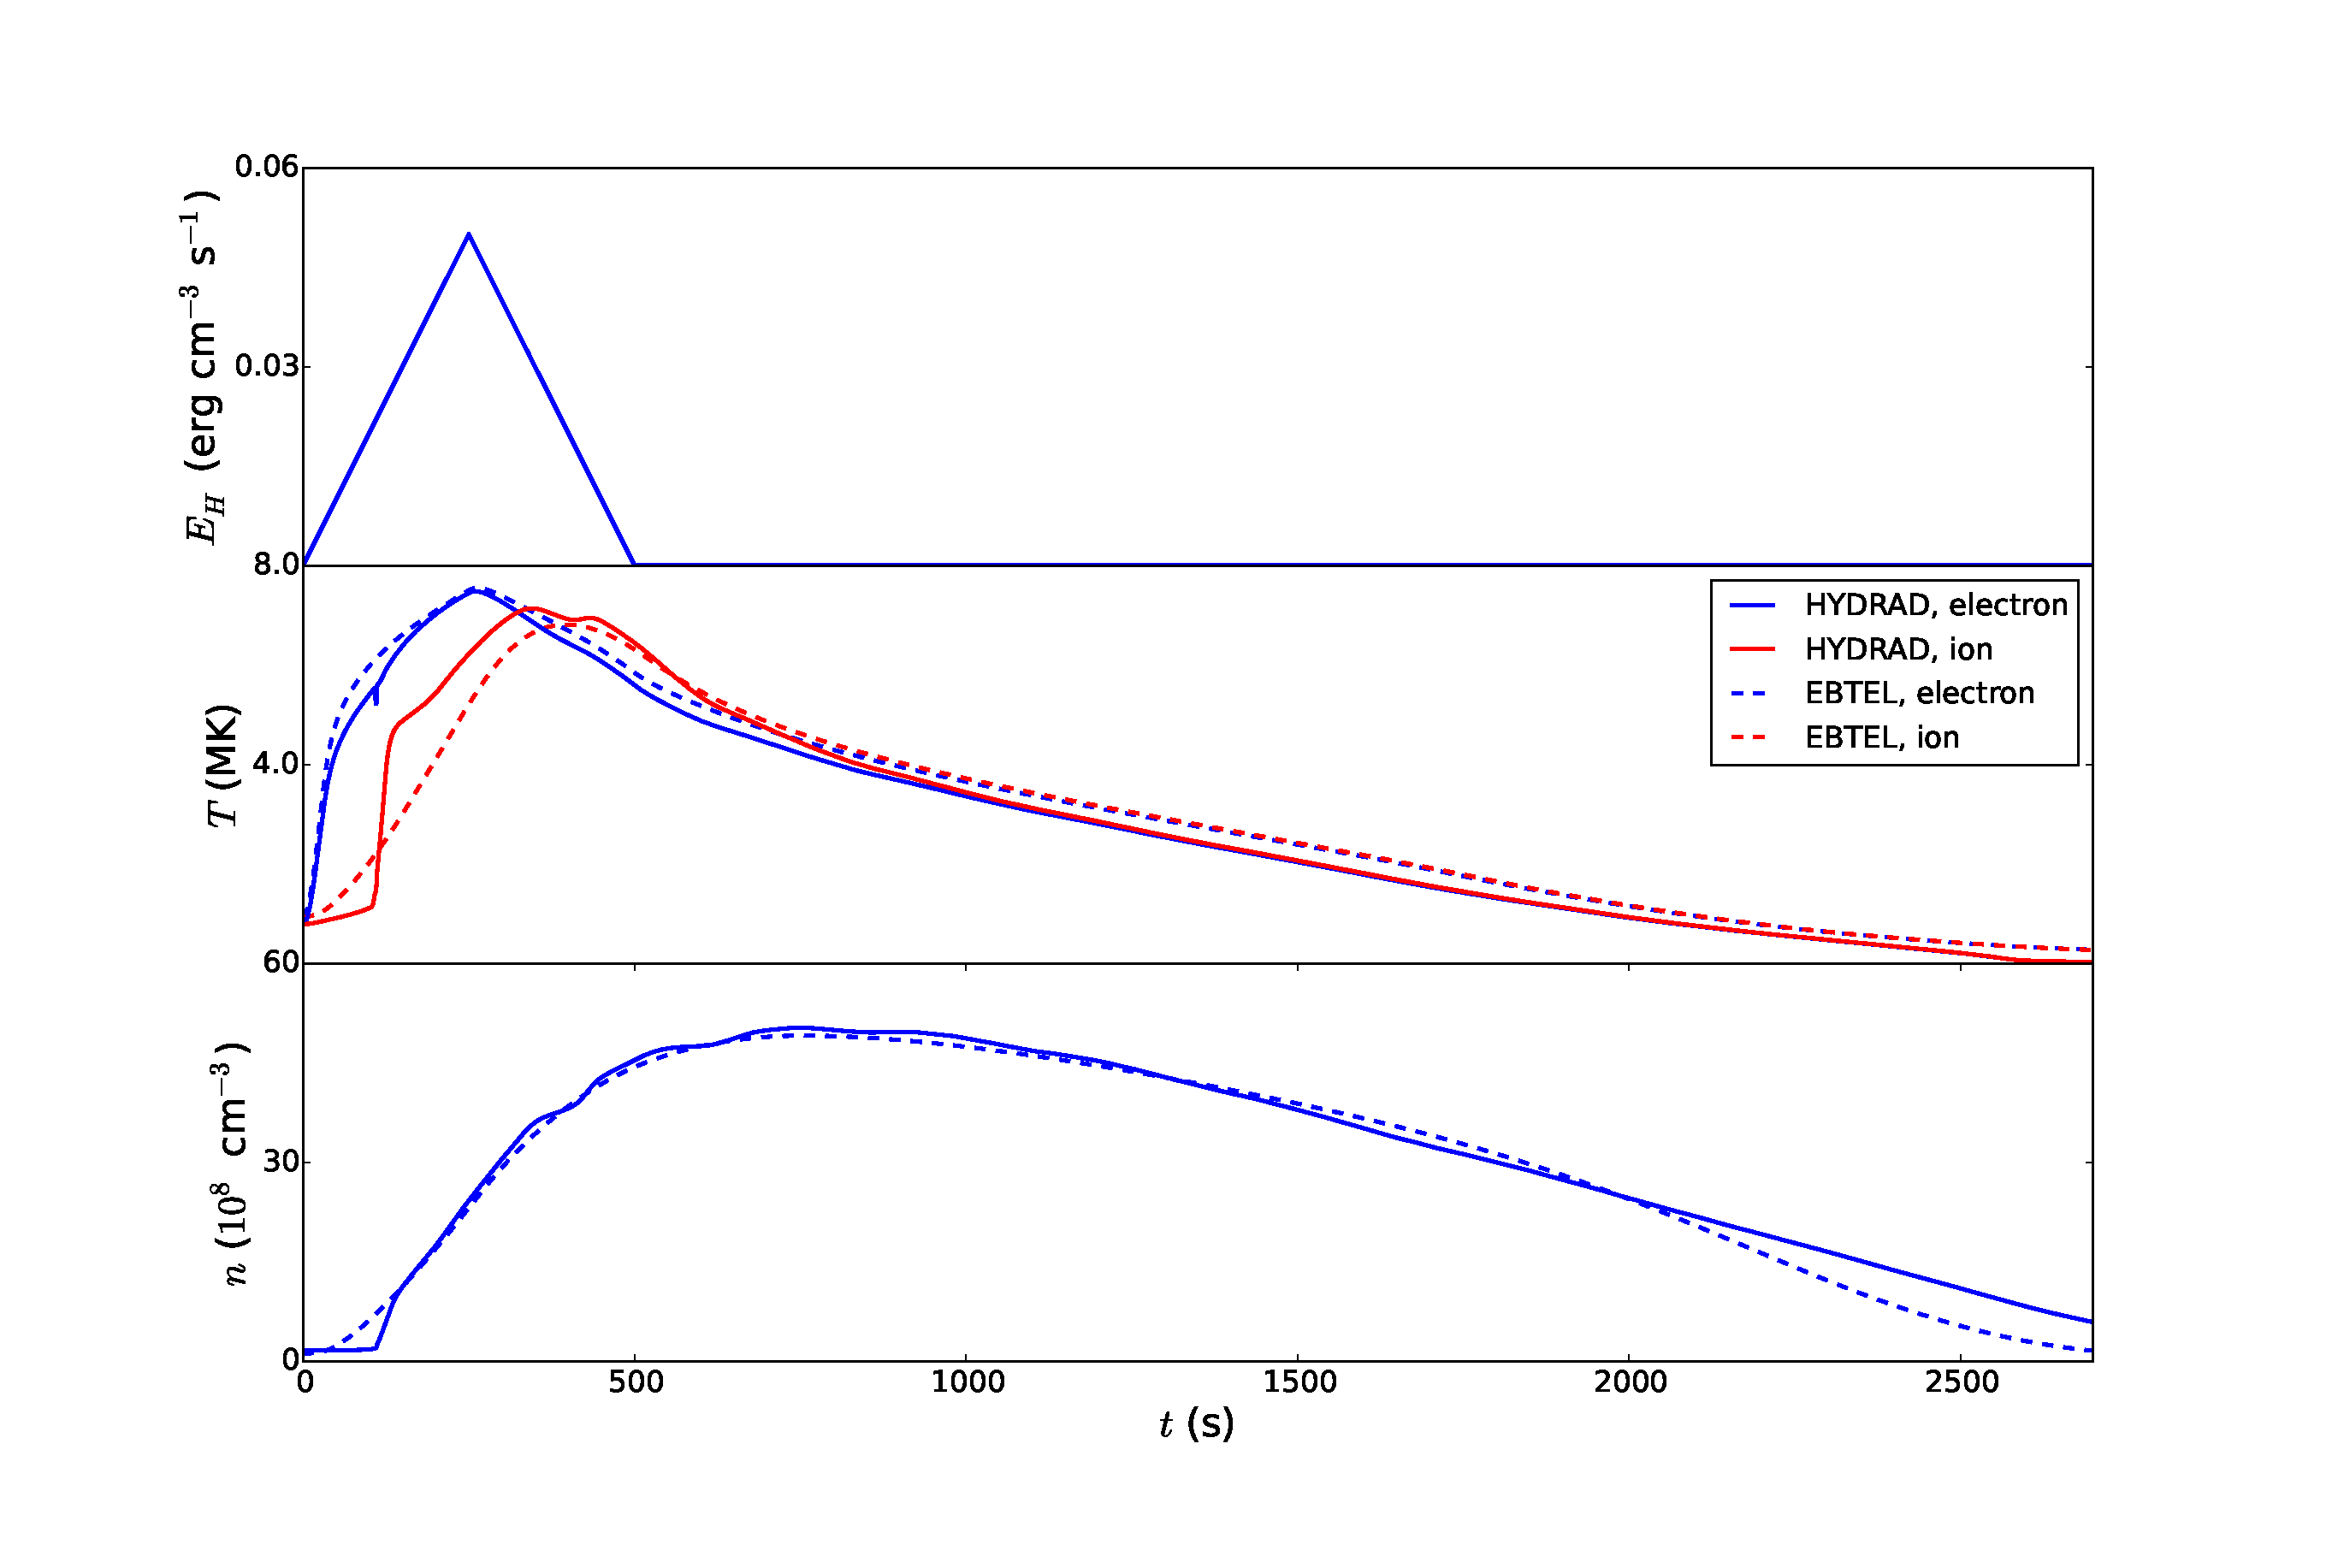
\includegraphics[width=0.85\textwidth]{figures/ebtel_tf_compare_1event.eps}
	\label{fig:ebtel_tf_compare_1}}
	\subfigure[]{%
	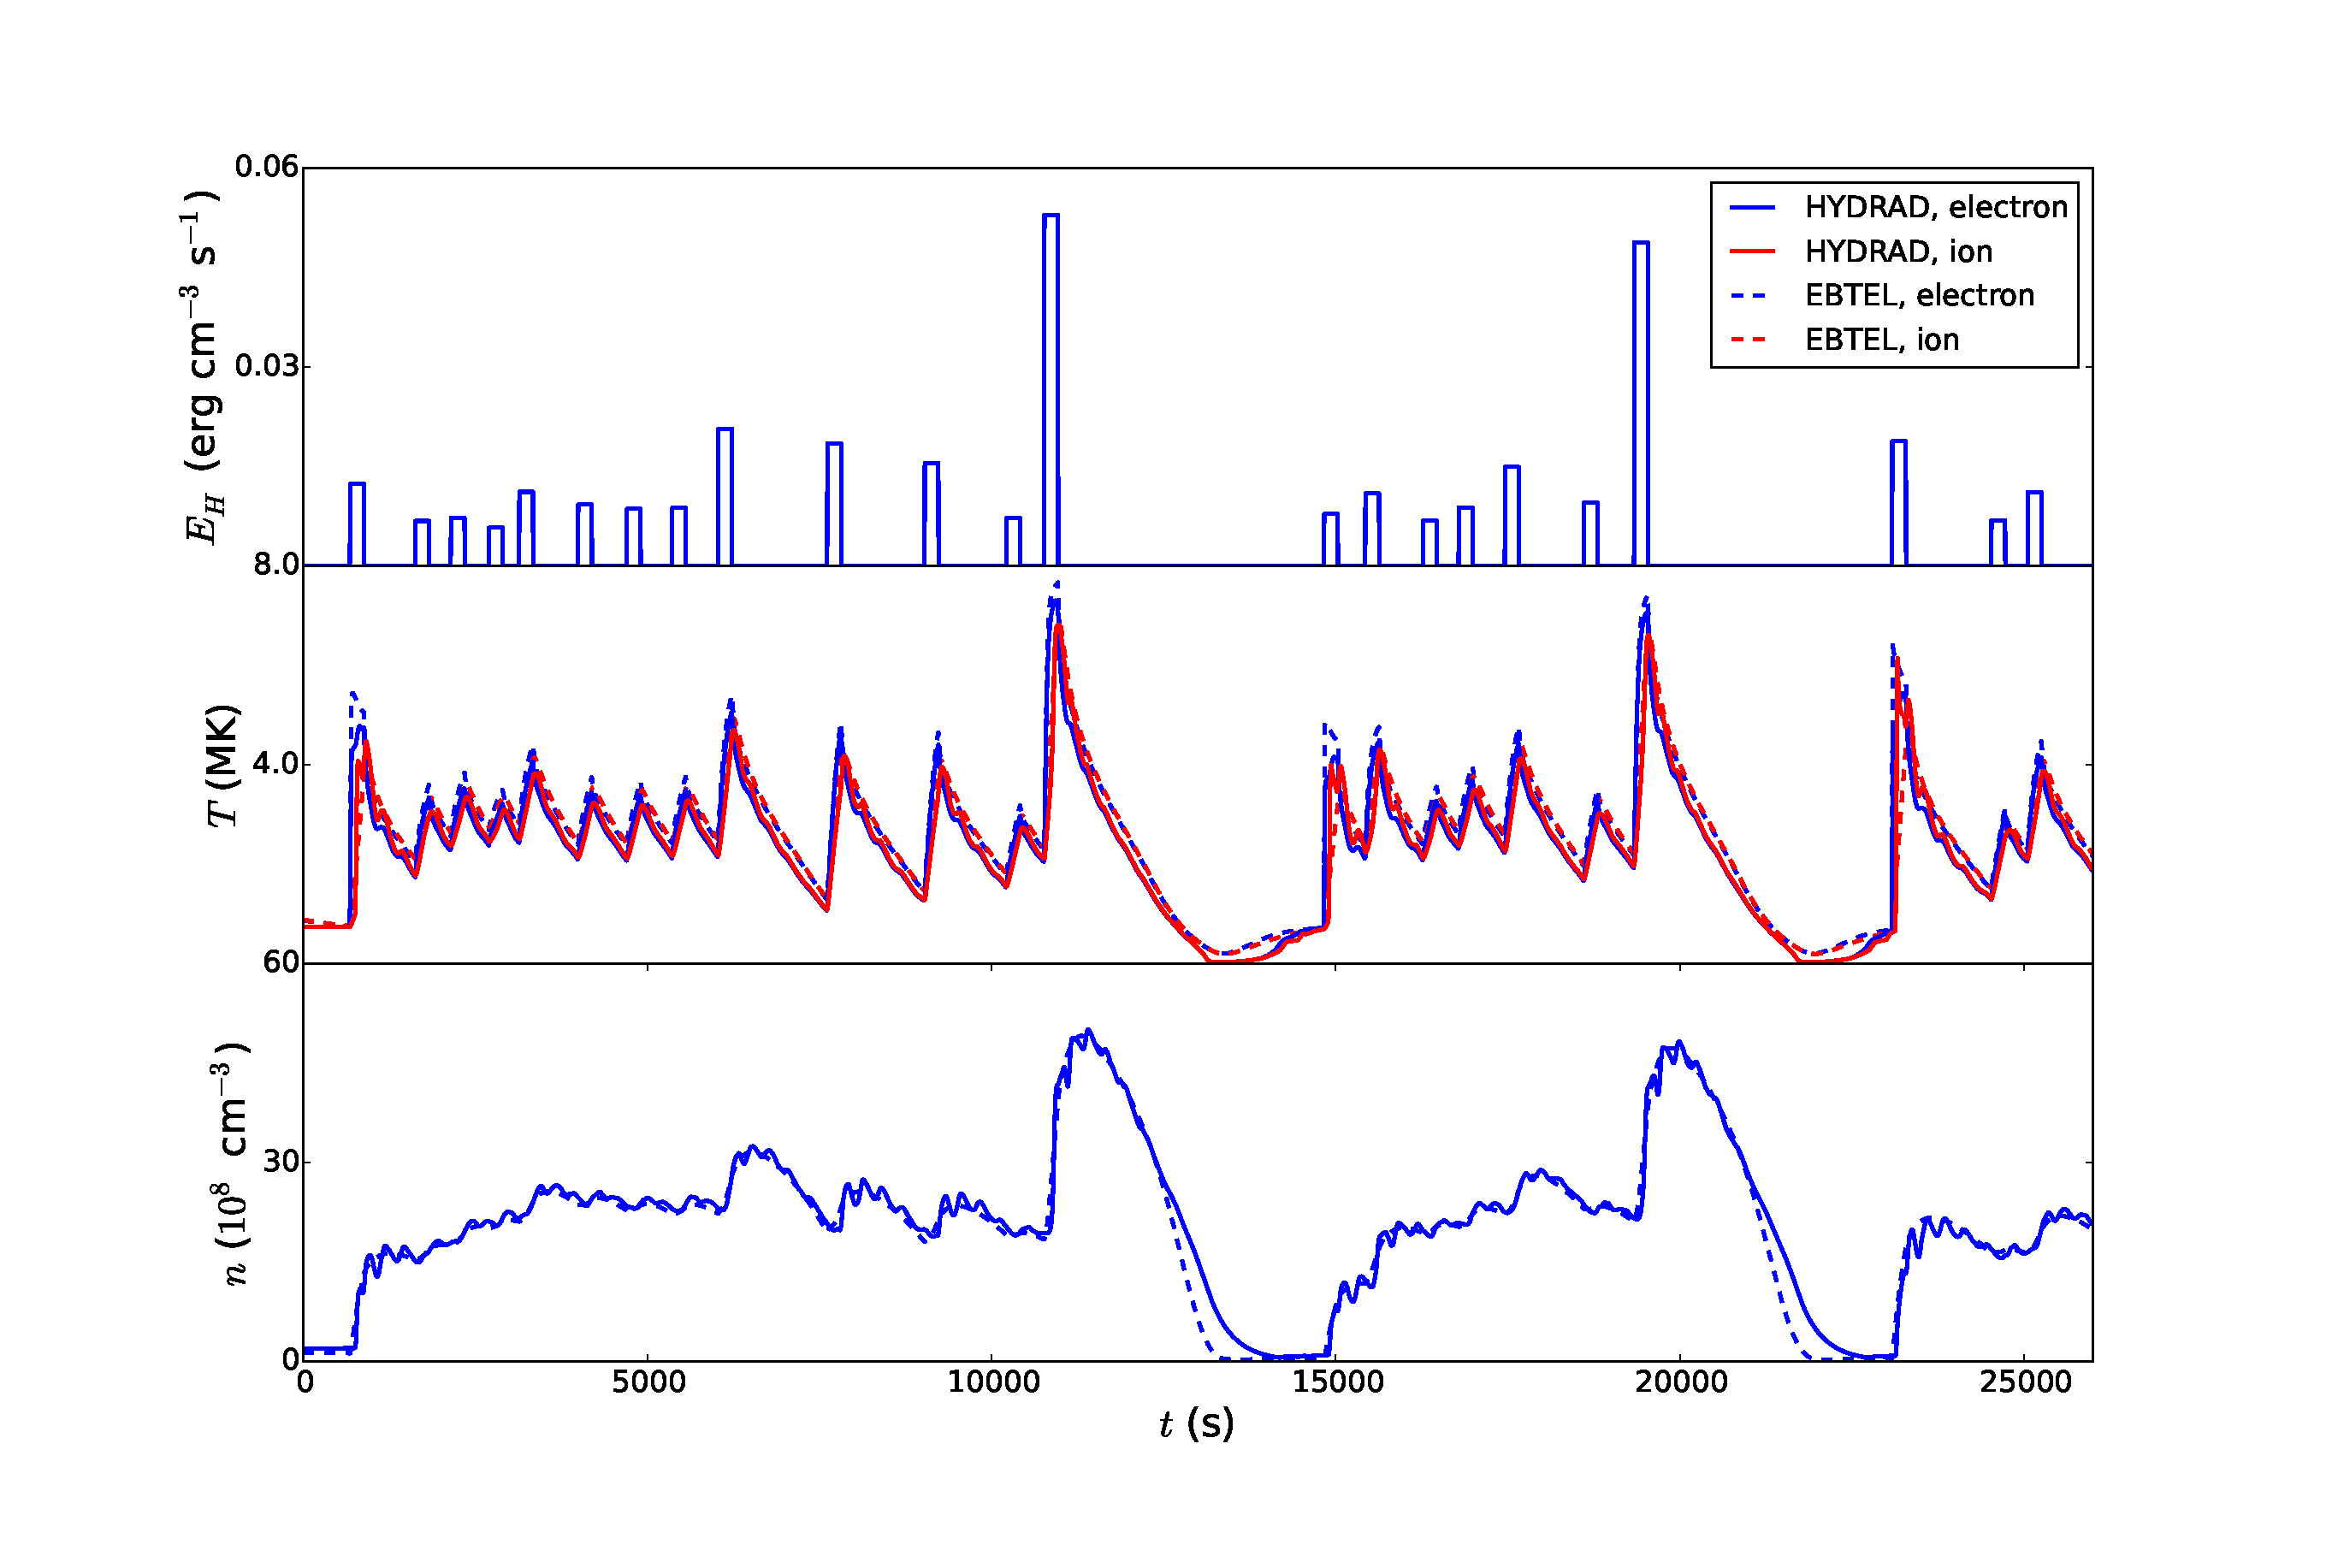
\includegraphics[width=0.85\textwidth]{figures/ebtel_tf_compare_manyevents.eps}
	\label{fig:ebtel_tf_compare_m}}
	\caption{Comparisons between the EBTEL-2fl model (dashed) and HYDRAD (solid) for \textbf{(a)} a single triangular pulse lasting 500 s and \textbf{(b)} the same heating profile as in Fig. \ref{fig:ebtel_sf_compare}. The upper panels show the heating profiles, the middle panels show the electron (blue) and ion (red) temperature profiles, and the bottom panels show the density profiles.}
	\label{fig:ebtel_tf_compare}
\end{figure}
%
\par Looking back to Eqs. \ref{eq:ebtel2fl_press_e}, \ref{eq:ebtel2fl_press_i}, and \ref{eq:ebtel2fl_density}, one may notice that there are still two missing pieces: $\psi_C$ and $\psi_{TR}$. These terms arise from the spatial integrals over the electron pressure gradients that represent the the work done by the electric field on the species (the mobile electrons in this case) to maintain quasi-neutrality. To derive $\psi_{TR},$ first consider the quantity $\xi\equiv T_{e,0}/T_{i,0}.$ Then, using Eq. \ref{eq:pe_close}, multiplying by $1=v_0/v_0$, and again the approximation $p_{e,0}v_0\approx(p_ev)_0$, 
%
\begin{equation}
	\xi\equiv\frac{T_{e,0}}{T_{i,0}}=\frac{(p_ev)_0}{(p_iv)_0}.
\end{equation}
Plugging in Eqs. \ref{eq:enthalpy_flux_e} and \ref{eq:enthalpy_flux_i} and using a bit of algebra, an expression for $\psi_{TR}$ can be derived,
\begin{equation}
	\label{eq:psi_tr}
	\psi_{TR} = \frac{1}{1 + \xi}(F_{0,e} + \mathcal{R}_{TR} - \xi F_{0,i}).
\end{equation}
Additionally, $\psi_C$ is approximated as,
\begin{equation}
	\label{eq:psi_C}
	\psi_C = \int_C\mathrm{d}s~v\frac{\partial p_e}{\partial s}\approx \bar{v}p_e^{(a)} - (p_ev)_0.
\end{equation}
Thus, Eqs. \ref{eq:psi_tr} and \ref{eq:psi_C} provide the final pieces for the set of EBTEL-2fl equations. Additionally, note that, using Eq. \ref{eq:psi_tr}, $\psi_{TR} - F_{e,0} - \mathcal{R}_{TR}=-\xi(F_{i,0} + F_{e,0} + \mathcal{R}_{TR})/(1 + \xi)$. In the single-fluid limit, $\bar{T}_e=\bar{T}_i=\bar{T}$ or $\xi=1$, noting that $F_0=F_e + F_i$, it can be seen that $\psi_{TR} - F_{e,0} - \mathcal{R}_{TR}=-(F_0 + \mathcal{R}_{TR})/2$ such that the original EBTEL equation, Eq. \ref{eq:ebtel_sf_density} , is recovered from Eq. \ref{eq:ebtel2fl_density}. Thus, all three of the EBTEL-2fl equations reduce to the original single-fluid EBTEL equations in the limit of electron-ion equilibrium.
%
\par As with the original EBTEL model, EBTEL-2fl has been carefully benchmarked against the HYDRAD hydrodynamic code. Fig. \ref{fig:ebtel_tf_compare} shows a comparison between EBTEL-2fl and HYDRAD for two different heating functions. Fig. \ref{fig:ebtel_tf_compare_1} shows the responses of EBTEL-2fl and HYDRAD to a single triangular pulse with a duration of 500 s. Note that the density evolution matches quite well during both the heating phase and cooling phase. A noticeable discrepancy occurs between the two ion temperatures at the start of the heating phase. The EBTEL-2fl ion temperature tends to rise more quickly because the density increases more quickly, initially in the EBTEL model. Since the electron-ion coupling term $\propto n^2$, the ions couple more quickly to the heated electrons. This artificial density increase is a consequence of the 0D nature of the model: in a loop with spatial extent, there is an additional lag in the density increase due to the inertia of the plasma. However, in EBTEL-2fl, the ``loop'' has no spatial extent and so the plasma essentially begins moving up the loop in zero time. Additionally, \ref{fig:ebtel_tf_compare_m} shows the EBTEL-2fl response in density and temperature for a series of 200 s heating events. The $\bar{n},\bar{T}_e,\bar{T}_i$ profiles all track quite well relative to the HYDRAD profiles.
%
\section{Numerical Implementation}
\label{sec:numerical}
%
\par While the original EBTEL model of \citet{klimchuk_highly_2008,cargill_enthalpy-based_2012} was coded in the Interactive Data Language (IDL), a popular software package in solar physics, EBTEL-2fl has been implemented in the C programming language. The reason for this is twofold: 1) C offers a significant speedup over IDL, allowing for much more efficient parameter space explorations. For example, a 10,000 second run of the original EBTEL model can take up to 7 seconds, while an equivalent case in EBTEL-2fl takes only a fraction of a second. 2) C is freely available on all computing platforms while a department-wide IDL license could cost upwards of several hundred dollars. Since this code will eventually be distributed to the solar physics community, all researchers will be able to use the code regardless of the financial situation of their department or university. Additionally, C is in general more portable than proprietary languages like IDL, meaning that EBTEL-2fl can easily be run on large computing clusters, making parameter space investigations even more efficient. 
%
\par Though the original EBTEL code used only a simple Euler solver, with a static timestep, the EBTEL-2fl model includes a slightly more sophisticated solver with an optional adaptive timestepping routine. The code also includes an option to use a simple Euler. Below, both the Euler and fourth-order Runge-Kutta solvers will be briefly described. Additionally, details of the adaptive timestep routine will also be discussed.
%
\subsection{Euler Method}
\label{subsec:euler}
%
\par Perhaps the first step in any numerical ordinary differential equation (ODE) solution is the explicit Euler method. For an ODE of the form,
\begin{equation}
	\label{eq:nonlinear_ode}
	\frac{d y_i}{dt} = f(y_1(t),\ldots,y_i(t),\ldots,y_N(t);t),\quad y_i(t=0)=y_{i,0}\quad \text{for }i=1,\ldots,N,
\end{equation}
a first-order Euler solver for $y_i$ can be written as
\begin{equation}
	\label{eq:euler}
	y_{i,j+1} = y_{i,j} + \tau f(y_{1,j},\ldots,y_{i,j},\ldots,y_{N,j};t_j),
\end{equation}
where $\tau=t_{j+1}-t_j$ and $j$ is the index representing the current timestep. The index $i$ represents the number of quantities to be solved such that the right-hand side of Eq. \ref{eq:nonlinear_ode} can depend on all or none of the other quantities. In the case of the EBTEL-2fl model, $N=3$ and $y_1,y_2,y_3=p_e,p_i,n$. Note also that the EBTEL-2fl equations, Eqs. \ref{eq:ebtel2fl_press_e}, \ref{eq:ebtel2fl_press_i}, and \ref{eq:ebtel2fl_density} all have the format of Eq. \ref{eq:nonlinear_ode} with the values at $t=0$ being determined by static equilibrium conditions. 
\subsection{Fourth-order Runge-Kutta Method}
\label{subsec:rk4}
%
\par  While Euler solvers are easy to implement (see \S\ref{subsec:euler}) they often suffer from a lack of accuracy and stability \citep{press_numerical_1992}. Recall that for a first-oder Euler scheme, the global truncation error will be $\mathcal{O}(\tau)$. Thus, sufficiently small timesteps are needed to ensure an accurate solution. However, the smaller the timestep, the longer the compute time. The widely-used fourth-order Runge-Kutta method, RK4 hereafter, improves accuracy and stability by calculating the right-hand side of Eq. \ref{eq:nonlinear_ode} at intermediate points between $t$ and $t+\tau$. In particular, RK4 uses an Euler method to calculate the $f$ at $t+\tau/2$. The value of $y_i$ is then estimated at $t+\tau/2$ using this Euler method value of $f$ at $t+\tau/2$ and this new value of $y_i$ is used to estimate $f$ at $t+\tau$. The RK4 method for equations of the form of Eq. \ref{eq:nonlinear_ode} is given by,
\begin{equation}
	\label{eq:rk4}
	y_{i,j+1} = y_{i,j} + \frac{1}{6}(k_1 + 2k_2 + 2k_3 + k_4) + \mathcal{O}(\tau^5),
\end{equation}
where
\begin{align}
	k_1 &= \tau f(y_1(t_j),\ldots,y_N(t_j);t_j),\\[0.5em]
	k_2 &= \tau f(y_1(t_j) + k_1/2,\ldots,y_N(t_j) + k_1/2; t_j+\tau/2),\\[0.5em]
	k_3 &= \tau f(y_1(t_j) + k_2/2,\ldots,y_N(t_j) + k_2/2; t_j+\tau/2),\\[0.5em]
	k_4 &= \tau f(y_1(t_j) + k_3,\ldots,y_N(t_j) + k_3; t_j + \tau),
\end{align}
\citep{press_numerical_1992}. For a static timestep, where the total number of steps is $(\text{total time})/\tau$, the global truncation error will be $\mathcal{O}(h^4)$. Thus, Eqs. \ref{eq:ebtel2fl_press_e}, \ref{eq:ebtel2fl_press_i}, and \ref{eq:ebtel2fl_density} can be solved using Eq. \ref{eq:rk4} with greater accuracy than with Eq. \ref{eq:euler}.
%
\subsection{Adaptive Timestep Routine}
\label{subsec:adapt}
%
\par During the heating phase of a loop evolution cycle, particularly in an impulsive heating scenario, the temperature gradient in time can become very steep, especially if the density at the onset of heating is low (e.g. when the time between heating events is longer than the radiative cooling/draining timescale). Alternatively, during the radiative cooling phase, these temperature gradients are relatively shallow. Thus, very short timesteps will ensure adequate resolution of the behavior during the heating phase, but will lead to unnecessarily long compute times during the radiative cooling phase. On the other hand, using a long timestep will ensure small compute times, but could, at best, lead to an incorrect treatment of the fast-acting thermal conduction during the heating phase, and, at worst, cause serious stability issues in the solution during this period. 
%
\par Thus, Eqs. \ref{eq:ebtel2fl_press_e} and \ref{eq:ebtel2fl_press_i} lend themselves to an adaptive timestepping approach, where the timestep, $\tau$, is adjusted based on how the solution is changing at time $t_j$. There are many different timestepping control techniques; EBTEL-2fl uses the approach as outlined in \citet{garcia_numerical_2000}. Consider two cases of advancing the solution $y_{i,j}$ to $y_{i,j+1}$: 1) take one big timestep $\tau$ such that the final value is $y_{i,j+1}^{(b)}$; 2) take two small timesteps $\tau/2$ such that $y_i(t_j+\tau/2)$ is used to determined $y_i(t_j+\tau)=y_{i,j+1}^{(s)}$. 
%
\par To determine whether this error is acceptable, define $\Delta_c\equiv|y_{i,j+1}^{(b)} - y_{i,j+1}^{(s)}|$. Then, given some acceptable, user-specified error $\Delta_i$, the error ratio can be defined
\begin{equation}
	\epsilon = \frac{\Delta_c}{\Delta_i}.
\end{equation}
Recalling that the local truncation error for the RK4 method is $\Delta\propto\tau^5$, the new timestep can be defined as
\begin{equation}
	\tau_{new}=\tau\epsilon^{-1/5},
\end{equation}
where $\tau$ is the original timestep. If $\epsilon<1$, this new timestep is accepted. If $\epsilon>1$, the whole process is repeated with $\tau=\tau_{new}$. If the $\epsilon<1$ criteria is not met in some finite number of iterations, the routine fails.
%
\chapter{Results}
\label{ch:results}
This chapter will include the results of our numerical study
Here we will also describe how the study was performed and what tools were used to perform the study
It is best not to introduce any new tools here; just pool from those that have already been discussed and show how they were applied
Show lots of plots and tables
\chapter{Conclusions}
\label{ch:conclusions}
This chapter will discuss the conclusions that we can draw based on the results in the results section. What do these results mean? What are the implications in the context of loops in active region cores?
May include some topics for future work in this section as well or just wait and put it in a different chapter

\appendix

%\chapter{Coronal and Transition Region Pressure Gradient Integrals}
\label{ch:appendix}
% 
An appendix will go here.
%\appendix
%\addcontentsline{toc} {chapter}{\numberline {}Appendix A}
%\chapter{Coronal and Transition Region Pressure Gradient Integrals}
\label{ch:appendix}
% 
An appendix will go here.
%\chapter{Additional Plots}
\label{ch:appendix-b}
%
More plots will go here
%\addcontentsline{toc} {chapter}{\numberline {}Bibliography}{}
%\include{biblio}

\bibliographystyle{apj}
\bibliography{references.bib}
\end{document}
